%% Master Thesis Template
%% Please update the specification through this link: https://daim.idi.ntnu.no/howto_thesis_submission.pdf

\documentclass[pdftex,10pt,b5paper,twoside]{book}
\usepackage[lmargin=25mm,rmargin=25mm,tmargin=27mm,bmargin=30mm]{geometry}

\usepackage{setspace}
\usepackage{graphicx}
\usepackage{amssymb}
\usepackage{mathrsfs}
\usepackage{amsthm}
\usepackage{amsmath}
\usepackage{color}
\usepackage{csquotes}
\usepackage{subcaption}
\usepackage[Lenny]{fncychap}
\usepackage[pdftex,bookmarks=true]{hyperref}
\usepackage[pdftex]{hyperref}
\hypersetup{
    colorlinks,%
    citecolor=black,%
    filecolor=black,%
    linkcolor=black,%
    urlcolor=black
}
\usepackage[font=small,labelfont=bf]{caption}
\usepackage{fancyhdr}
\usepackage[acronym]{glossaries}
\usepackage{times}
\usepackage[square,sort,comma,numbers]{natbib}
\usepackage{float}
\usepackage{multicol}

\usepackage{grfext}
\PrependGraphicsExtensions*{.pdf}

%\floatstyle{boxed} 
\restylefloat{figure}

\renewcommand*\contentsname{Table of Contents}

\pagestyle{fancy}
\fancyhf{}
\renewcommand{\chaptermark}[1]{\markboth{\chaptername\ \thechapter.\ #1}{}}
\renewcommand{\sectionmark}[1]{\markright{\thesection\ #1}}
\renewcommand{\headrulewidth}{0.1ex}
\renewcommand{\footrulewidth}{0.1ex}
\fancypagestyle{plain}{\fancyhf{}\fancyfoot[LE,RO]{\thepage}\renewcommand{\headrulewidth}{0ex}}

\newacronym{CA}{CA}{Cellular automaton (pl. automata)}

\makeglossaries


\begin{document}

\frontmatter

%% PART 1
%%The title page will be automatically generated and added by the DAIM system
%\vspace*{7cm}
\begin{center}

\emph{dedication (optional)}

\end{center}

\cleardoublepage		%% Optional

%% PART 2
\clearpage
\pagenumbering{roman} 				
\setcounter{page}{1}

\pagestyle{fancy}
\fancyhf{}
\renewcommand{\chaptermark}[1]{\markboth{\chaptername\ \thechapter.\ #1}{}}
\renewcommand{\sectionmark}[1]{\markright{\thesection\ #1}}
\renewcommand{\headrulewidth}{0.1ex}
\renewcommand{\footrulewidth}{0.1ex}
\fancyfoot[LE,RO]{\thepage}
\fancypagestyle{plain}{\fancyhf{}\fancyfoot[LE,RO]{\thepage}\renewcommand{\headrulewidth}{0ex}}

\section*{\Huge Summary}
\addcontentsline{toc}{chapter}{Summary}	
$\\[0.5cm]$

\noindent Write your summary here...

\clearpage		%% Optional
\section*{\Huge Preface}
\addcontentsline{toc}{chapter}{Preface}
$\\[0.5cm]$

\noindent Write your preface here...

\cleardoublepage		%% Optional
\tableofcontents
\addcontentsline{toc}{chapter}{Table of Contents}
\clearpage

\listoftables
\addcontentsline{toc}{chapter}{List of Tables}
\clearpage

\listoffigures									
\addcontentsline{toc}{chapter}{List of Figures}
\clearpage			%% Generate TOC, list of tables, and list of figures automatically
%\section*{{\Huge Abbreviations}}
\addcontentsline{toc}{chapter}{Abbreviations}
$\\[0.5cm]$

\printglossary[title=Abbreviations]
	%% Optional

\cleardoublepage

\pagestyle{fancy}
\fancyhf{}
\renewcommand{\chaptermark}[1]{\markboth{\chaptername\ \thechapter.\ #1}{}}
\renewcommand{\sectionmark}[1]{\markright{\thesection\ #1}}
\renewcommand{\headrulewidth}{0.1ex}
\renewcommand{\footrulewidth}{0.1ex}
\fancyfoot[LE,RO]{\thepage}
\fancyhead[LE]{\leftmark}
\fancyhead[RO]{\rightmark}
\fancypagestyle{plain}{\fancyhf{}\fancyfoot[LE,RO]{\thepage}\renewcommand{\headrulewidth}{0ex}}

\mainmatter

%% PART 3 -- The Chapters
\chapter{Introduction}
\textit{Cellular Automata} (CA) were first conceptualized and introduced in the 1940's and 1950's.
Around the same time, the idea of the \textit{evolutionary algorithm} was also being developed independently.
Both of these concepts take inspiration from nature, and thus fall into the category of \textit{artificial life}.
One goal of this field of research is to create systems that are of complexity comparable to that of biological systems found in nature.

One way to try to achieve this goal is to combine these two distinct concepts: Cellular systems designed by evolution.
Many different kinds of tasks have been solved by cellular systems that have been created this way.
However, more complex tasks and more complex models means greater spaces of possible solutions that the evolutionary algorithm must search.
%This phenomenon is seen in many fields, and is often referred to as "the curse of dimensionality" (TODO citation).
For a traditional genetic algorithm it can be both time consuming and challenging to find good solutions.

One of the possible ways to remedy this problem is to replace the traditional table-based encoding of CA transition rules with a different encoding: an encoding that supports a more complex evolutionary algorithm.
This paper describes the investigation of using \textit{Compositional Pattern Producing Networks} (CPPNs) as the data structure for transition rules,
and the \textit{NeuroEvolution of Augmenting Topologies} (NEAT) genetic algorithm for evolving these CPPNs.

With CPPN-based transition functions there is not a linear relationship between the input-output size and the size of the encoding.
The algorithm starts with the smallest possible encoding and iteratively over time adds features to it and adjusts them until an optimal solution is found.
This \textit{complexification} mimics the process that biologists believe life on earth developed.

To test this new combination, which we call \textit{CA-NEAT},
a custom Python framework was built to run simulations in software.
The framework was tasked with solving various CA tasks of different difficulties, with different degrees of success.

TODO research question

TODO outline thesis

\cleardoublepage
\chapter{Background \& Motivation}
\section{Complex and Biologically-Inspired Systems}
\epigraph
{
If you try and take a cat apart to see how it works, the first thing you have on your hands is a nonworking cat.
}
{Douglas N. Adams \\ \textit{The Salmon of Doubt} \cite{adams2002salmon}}

\begin{figure}
\centering
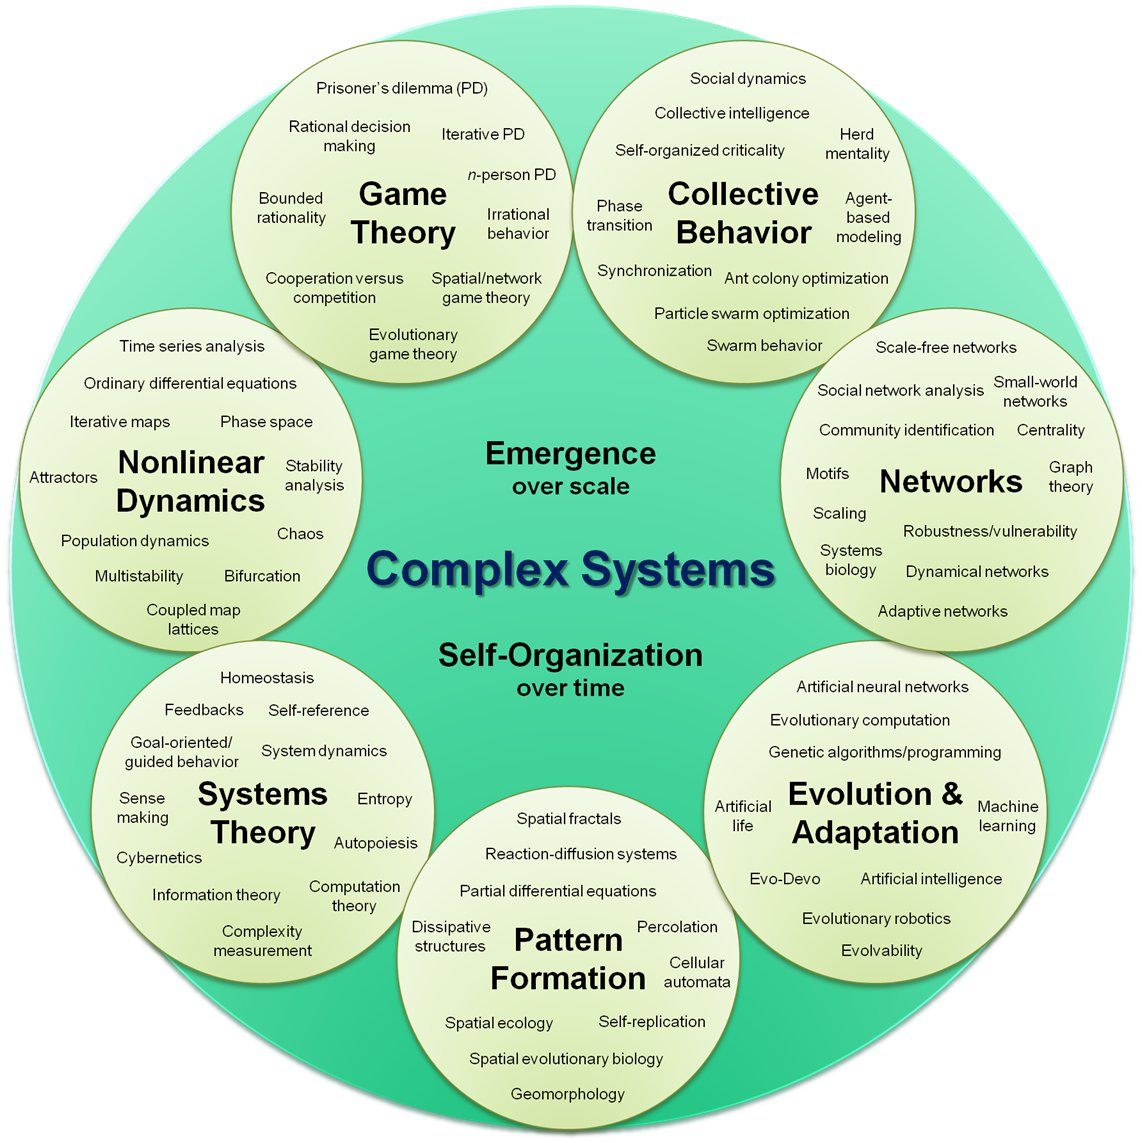
\includegraphics[width=.65\textwidth]{fig/complex_systems_sayama}
\caption[Complex systems taxonomy]{Complex systems taxonomy. Reproduced from \cite{sayama2015introduction} by Hiroki Sayama. TODO check that this figure is readable when printed B5}
\label{fig:complex_systems_taxonomy}
\end{figure}

\textit{Complex systems} is an umbrella category consisting of a variety of topics from a variety of domains, such as mathematics, computer science and biology.
Figure \ref{fig:complex_systems_taxonomy} shows one possible "taxonomy" of complex systems.
It is not immediately obvious why these topics should be grouped together.
The word \textit{complex} is related to \textit{complicated}, synonymous with \textit{difficult}, \textit{intricate} and \textit{perplexing} \cite{Thesaurus.com2017}.
In 1962, Herbert Simon proposed a definition as \textquote[\cite{simon1962architecture}]{made up of a large number of parts that interact in a non-simple way}.
Hiroki Sayama later elaborated this definition:
\blockquote[\cite{sayama2015introduction}]{
Complex systems are networks made of a number of components that interact with each other, typically in a nonlinear fashion.
Complex systems may arise and evolve through self-organization, such that they are neither completely regular nor completely random, permitting the development of emergent behavior at macroscopic scales.
}
By grouping these topics together,
it is possible to start seeing similarities across domains,
and find insights about one topic that may be applicable to other topics.

A common property of complex systems is \textit{emergence} over scale.
Sayama defines emergence as \textquote{a nontrivial relationship between the properties of a system at microscopic and macroscopic level}.
This means that a process which can be observed at the macroscopic level (e.g. the human body moving) can not be explained by studying the individual components that make up the system (looking at the cells that make up the body).
Instead, both the individual components and \textit{how they interact} must be understood.

The other common property of complex systems is \textit{self-organization} over time.
Sayama defines it as \textquote{a dynamical process by which a system spontaneously forms nontrivial macroscopic structures and/or behaviors over time}.
One example is magnetization of metals, where the initially random configuration of "spins" (the components of the larger system) orient themselves over time,
so that the magnetic vector of all the individual spins and that of the whole system become the same \cite{heylighen2001science}.

The behavior seen in complex systems can be characterized by these two properties.
Often the behavior is a combination of the two properties, rather than a clear instance of one or the other.

%Complex systems may have parameters that affect the outcome of the process they partake in.
%The term \textit{equifinality} is used to describe systems of different configurations that arrive at the same result TODO cite.

Many of the topics seen in Figure \ref{fig:complex_systems_taxonomy} are based on concepts found in nature.
These belong to the group of \textit{bio-inspired systems} and to the category of \textit{artificial life}.
Since the infancy of modern computing in the 1940s, computers have gradually gained the capability to perform many tasks.
Along the way, computer scientists and engineers have sometimes looked to nature for inspiration and goals to reach for.
Many times approaching problems from engineering, mathematical and logical perspectives have yielded good results.
But some times, the analytical approach leads to a dead end.
Some tasks that are trivial for a human to perform, can be practically impossible for a programmer to codify \cite{moravec1988mind}.
This is where the bio-inspired approach may help.
Since nature has been able to create biological "machines" that can solve these tasks, then perhaps borrowing nature's methods will allow computers to do the same.

\subsection{Morphogenetic Engineering}
The field of \textit{morphogenetic engineering} \cite{doursat2013review} studies the confluence between biological and artificial systems, and how to create new systems that straddle the the divide.
Doursat et. al. defined four categories of morphogenetic engineering that they classified existing techniques by:

\begin{description}
    \item[Category I: by Constructing] ~\\
        e.g. self-assembling robots
    \item[Category II: by Coalescing] ~\\
        e.g. swarm agents
    \item[Category III: by Developing] ~\\
        e.g. genetic algorithms
    \item[Category IV: by Generating] ~\\
        e.g. bio-inspired grammars
\end{description}

Within the third category we find many of the concepts that this thesis is concerned with, such as evo-devo and morphogenesis.

\section{Cellular Automata}
\textit{Cellular Automata} (CA) were first invented in the 1940s by John von Neumann and Stanislaw Ulam as mathematical models of computation \cite{von-neumann-1966}.
They were inspired by biological organisms,
and created a model that could emulate some of their interesting and useful properties,
such as multi-cellular development (e.g. embryogenesis), reproduction (clonal or sexual) and robustness (e.g. self-repair).

In the following decades, as modern computers emerged,
the concept of CA became the basis for the field of \textit{Cellular Computing} (CC).
As the performance of "conventional" computers kept increasing dramatically (as described by \textit{Moore's law})\cite{schaller1997moore},
CC never became the basis for the mainstream computers that we use today,
but CA and CC remained an area of research by mathematicians and computer scientists,
and as part of the larger field of artificial life.
More recently, as Moore's law has faltered and this rate of growth of performance has diminished,
some have started to look for new methods that can lead to renewed performance growth.
Parallel computing has helped a lot, but it has shown itself to be difficult in practice.
Some, such as Michael J. Flynn have speculated that CC might be the path forward \cite{flynn-1996} .
Matthew Cook proved that a CA of a certain configuration can be Turing complete \cite{cook-2004},
giving further credibility to this idea.

\subsection{CA Definition}
A CA consists of a grid of very simple units called cells.
A cell can be in one out of a finite set of states, and can change between states based on input to the cell.
As such the CA can be considered as a grid of identical Finite State Automatons.
Sipper \cite{sipper-1999} described the three core principles of CC, which also apply to CA in general:

\begin{description}
    \item[Simplicity]
        ~\\
        A cell is simple and can do very little by itself.
    \item[Vast Parallelism]
        ~\\
        The number of cells is very large, much more than the number of processors in a conventional parallel computer.
    \item[Locality]
        ~\\
        All interactions between cells take place on a purely local basis.
        No cell knows or controls the entire system.
\end{description}

The cells in a CA can "see" only their closest neighboring cells.
They use this limited information in conjunction with some set of rules to transition from one cell state to another.
Depending on the starting state of the whole system and the rules,
it is possible to observe interesting emergent or self-organizing behavior over time and space.
These interesting CA often find an \textit{attractor} \cite{gershenson-2004, wolfram1986theory}.
If a sequence of CA states repeat periodically it is called a \textit{cycle attractor}, and if the CA stabilizes into a permanent, fixed state is is called a \textit{point attractor}.
Figure \ref{fig:example_CA} shows an example of a CA that enters a cyclical attractor.
Binary CA, with only two possible cell states, are the most commonly seen and studied.
Greater numbers of cell states is possible, but the increase in degrees of freedom can lead to some problems.

\begin{figure}[h]
\centering
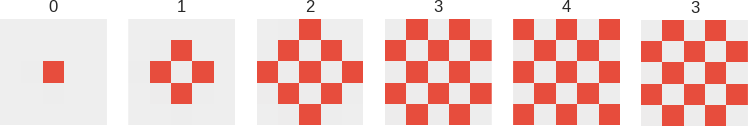
\includegraphics[height=0.4\textheight, width=\textwidth, keepaspectratio]{fig/result_figs/generate_mosaic/1}
\caption[Example CA]{An example binary 2D CA. At time step 5 the CA state is the same as that in time step 3, meaning the CA has entered a cyclical attractor with a period of 2 (oscillation).}
\label{fig:example_CA}
\end{figure}

%There are many properties of CA and of cellular computing that can be varied to produce different results \cite{sipper-1999}.
%In this paper we will define some further properties of CA as:
%\begin{itemize}
%    \item Structured as a 1D or 2D cartesian grid of cells.
%    \item Having uniform cells, sharing the same transition rules.
%    \item Having a finite discrete set of states that cells can have.
%    \item Synchronously changing states for all cells.
%\end{itemize}

%Examples that fit into this narrower definition include Von Neumann's cellular automaton \cite{von-neumann-1966}, Wolfram's elementary cellular automata (TODO cite) and Conway's Game of Life (TODO cite Conway).

%Figure \ref{fig:110} illustrates "elementarty CA 110", which has this property.
%This is an 1D CA, with successive states transitioning from the top to the bottom over time.
%Two different patterns stand out from the background.
%Over time they move towards each other and interact.
%This interaction is used in Cook's proof that CA 110 is Turing complete.
%
%\begin{figure}
%\centering
%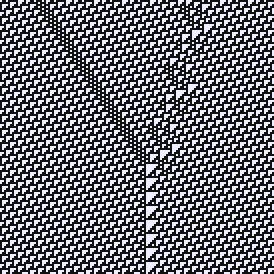
\includegraphics[width=\columnwidth]{fig/110}
%\caption{Elementary CA 110
%(TODO cite \protect\url{https://commons.wikimedia.org/wiki/File:Ca110-interaction.png} properly)}
%\label{fig:110}
%\end{figure}

%Since the inception of CA by Ulam and Von Neumann in the 1940s \cite{von-neumann-1966},
%researchers have been interested in them for their biology-like properties and emergent behavior.
%Most implementations of CA have been formal mathematical works or simulations on conventional computers,
%but work has also been done with physical implementations using various substrates (TODO cite).
%
%In recent times the problem posed by the end of Moore's law and he difficulty of parallel computing with conventional architectures has caused cellular computing to become relevant again.
%Michael J. Flynn created Flynn's Taxonomy in 1966 \cite{flynn-1966}, describing different types of parallel systems.
%In 1996 he wrote a new article \cite{flynn-1996},
%outlining some of the difficulties that had hindered the expected parallel processing power that he and his peers had imagined back then.
%In this article he also described what he thought to be the road ahead, which is to represent problems in cellular form.

\subsection{Transition Rules}
\label{sec:transitions}
Langton \cite{langton-1990} formally defined finite CA as consisting of a finite set of cell states $\Sigma$ of size $K = |\Sigma|$,
a finite input alphabet $\alpha$, and a transition function $\Delta$.
Each cell has a $N$-sized neighborhood.
The number of possible neighborhood states can be expressed by equation \eqref{eq:kn}.

\begin{equation}\label{eq:kn}
    |\alpha| = |\Delta| = |\Sigma^N| = K^N
\end{equation}

The transition function for a CA must thus encode $|\alpha|$ different mappings of $N$ inputs to one of $K$ outputs.
The number of possible unique transition function behaviors is thus $K^{(K^N)}$.

\begin{figure}
\centering
\begin{subfigure}[t]{.175\columnwidth}
\centering
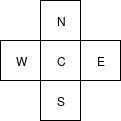
\includegraphics[width=\columnwidth]{fig/VonNeumann}
\caption{$N=5$ (Von Neumann)}
\label{fig:neighborhoods_vn}
\end{subfigure}\hfill%
\begin{subfigure}[t]{.175\columnwidth}
\centering
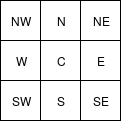
\includegraphics[width=\columnwidth]{fig/Moore}
\caption{$N=9$ (Moore)}
\end{subfigure}\hfill%
\begin{subfigure}[t]{.175\columnwidth}
\centering
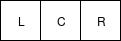
\includegraphics[width=\columnwidth]{fig/LCR}
\caption{$N=3$}
\end{subfigure}\hfill%
\begin{subfigure}[t]{.40\columnwidth}
\centering
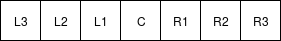
\includegraphics[width=\columnwidth]{fig/LLLCRRR}
\caption{$N=7$}
\end{subfigure}\hfill%

\caption[Some CA neighborhoods]{Some examples of common neighborhood shapes. The two common 2D shapes are named for John von Neumann and Edward F. Moore.
}
\label{fig:neighborhoods}
\end{figure}

\subsection{The $\lambda$ Parameter and the Edge of Chaos}
When Christopher Langton studied the elementary CA ($N=3, K=2$) \cite{langton-1990},
he created a metric to help determine if a rule is ordered, chaotic, or something in between, which he called $\lambda$.
It is defined by $K$, $N$ and the number of transitions that goes to the quiescent state, $n$.
\begin{equation}\label{eq:lambda}
    \lambda = \frac{K^N - n}{K^N}
\end{equation}

Langton found that low elementary CA $\lambda$ values resulted in ordered behavior, either settling into a static state or repeating periodically.
With high $\lambda$ values, the CA became chaotic, losing all useful information in the noise.
But at the critical border region between order and chaos, interesting behaviors and computation could occur \cite{langton-1990}.
This area has come to be called the \textit{edge of chaos}.

In the study Langton investigated the $\lambda$ of 1D binary CA, but the measure can be used on any CA.
The 2D binary transition function shown in Table \ref{tbl:example_CA} has 17 input combinations that lead to the quiescent ($0$) state ($n = 17$), and thus $\lambda \approx 0.47$.

\subsection{Finding Interesting Transition Functions}
\label{sec:finding_transitions}
\begin{table}
    \centering
    \caption[Example table-based transition rule]{
        An example table-based transition rule that exhibits the same behavior as seen in Figure \ref{fig:example_CA}.
        $N=5, K=2$ gives $|\alpha|=32$, the height of the table.
        The neighborhood shape is "Von Neumann" (Figure \ref{fig:neighborhoods_vn}).}
    \begin{tabular}{ccccc|c}
    North ($t_0$) & West ($t_0$) & Center ($t_0$) & East ($t_0$) & South ($t_0$) & Center ($t_1$) \\ \hline
    0      & 0      & 0      & 0      & 0      & 0        \\
    0      & 0      & 0      & 0      & 1      & 1        \\
    0      & 0      & 0      & 1      & 0      & 1        \\
    0      & 0      & 0      & 1      & 1      & 1        \\
    0      & 0      & 1      & 0      & 0      & 0        \\
    0      & 0      & 1      & 0      & 1      & 0        \\
    0      & 0      & 1      & 1      & 0      & 0        \\
    0      & 0      & 1      & 1      & 1      & 0        \\
    0      & 1      & 0      & 0      & 0      & 1        \\
    0      & 1      & 0      & 0      & 1      & 1        \\
    0      & 1      & 0      & 1      & 0      & 1        \\
    0      & 1      & 0      & 1      & 1      & 1        \\
    0      & 1      & 1      & 0      & 0      & 0        \\
    0      & 1      & 1      & 0      & 1      & 0        \\
    0      & 1      & 1      & 1      & 0      & 0        \\
    0      & 1      & 1      & 1      & 1      & 0        \\
    1      & 0      & 0      & 0      & 0      & 1        \\
    1      & 0      & 0      & 0      & 1      & 1        \\
    1      & 0      & 0      & 1      & 0      & 1        \\
    1      & 0      & 0      & 1      & 1      & 1        \\
    1      & 0      & 1      & 0      & 0      & 0        \\
    1      & 0      & 1      & 0      & 1      & 0        \\
    1      & 0      & 1      & 1      & 0      & 0        \\
    1      & 0      & 1      & 1      & 1      & 0        \\
    1      & 1      & 0      & 0      & 0      & 1        \\
    1      & 1      & 0      & 0      & 1      & 1        \\
    1      & 1      & 0      & 1      & 0      & 1        \\
    1      & 1      & 0      & 1      & 1      & 1        \\
    1      & 1      & 1      & 0      & 0      & 0        \\
    1      & 1      & 1      & 0      & 1      & 0        \\
    1      & 1      & 1      & 1      & 0      & 0        \\
    1      & 1      & 1      & 1      & 1      & 0        \\
    \end{tabular}
    \label{tbl:example_CA}
\end{table}

Traditionally $\Delta$ has been encoded as a complete mapping $\Delta: \Sigma^N \rightarrow \Sigma$, which can be implemented as a lookup table.
Table \ref{tbl:example_CA} shows an example of a table encoding for the CA in Figure \ref{fig:example_CA}.
This works very well for smaller cases such as the elementary CA.
But when working with non-trivial CA where both $K$ and $N$ can be relatively large numbers,
it becomes a problem both to store the mapping $\Delta$ in an efficient way,
and the space of possible $\Delta$ becomes too large to be explored by exhaustive enumeration.

Designing $\Delta$ with interesting behavior by hand is possible,
but it is time-consuming and impractical for problems of greater dimensions.
Using adaptive algorithms to explore the space of possible solutions is more feasible.
This is not guaranteed to produce good results though.
The use of table-based encodings put certain limitations on the search.
Using other encodings may enable new, more powerful search algorithms.
%This thesis concerns the investigation of a novel transition function encoding and associated search algorithm.

%\subsection{CA Problems}
%There are many kinds of problems that can be solved with CA.
%One class of problems is called \textit{morphology problems}.
%In these problems, the goal is for the CA to create some kind of complex structure.
%This can for example be \textit{morphogenesis}, where a simple structure is over time transformed into a more complex one,
%or it can be \textit{replication}, where some complex structure present initially must be copied.
%
%Another class of problems can be called \textit{information problems} (TODO is there a more appropriate term?).
%In this kind of problem the goal can be to compute some result based on the initial state, or to transmit information about state from one end to another.
%
%TODO citations

\section{Artificial Neural Networks}
\begin{figure}
\centering
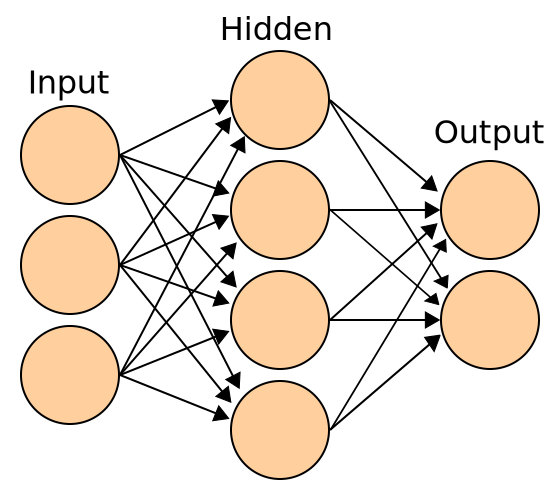
\includegraphics[width=.5\columnwidth]{fig/Artificial_neural_network}
\caption[Example ANN]{
    An example layered ANN with three input neurons, one bias neuron, three hidden neurons and two output neurons.
    Each connection between neurons also has some weight that scales the value being passed (not shown).
}
\label{fig:ann}
\end{figure}

\textit{Artificial Neural Networks} (ANNs) \cite[Chapter 1]{bengio2015deep} have been used in many different applications related to artificial life and intelligence,
such as robotics or machine learning.
An ANN is a directed graph structure, with vertices (referred to as neurons) and edges (referred to as connections).
Input values are fed into the first layer of neurons and passed through the connections to the next layers.
All the connections to one neuron is added together and input to the neuron.
In each neuron some activation function transforms the input to a new value, and in each connection the value is scaled by some weight.
There can also be \textit{bias} neurons, outputting values that are constant, not determined by input.

This is inspired by neuroscience, with the brain consisting of neurons and synapse connections.
ANNs are useful because they consists of many discrete parts that can be individually or collectively tuned by some adaptive process,
and are easily expanded.
The \textit{universal approximation theorem} \cite{Hornik1989359} shows that relatively simple ANNs can approximate a wide variety of functions,
and the field of deep learning shows that a large complex structure with enough tuning can perform very complex tasks, such as image classification or natural language processing.
Figure \ref{fig:ann} shows an example ANN with three inputs and two outputs.
An example of a use case for this structure could be to control a robot with three sensors and two motors.

\subsection{Compositional Pattern Producing Networks}
\begin{figure}
\centering
\begin{subfigure}[b]{.25\columnwidth}
\centering
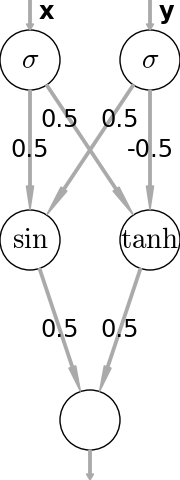
\includegraphics[height=5cm, keepaspectratio]{fig/2-cppn}
\caption{~}
\end{subfigure}\hfill%
\begin{subfigure}[b]{.65\columnwidth}
\centering
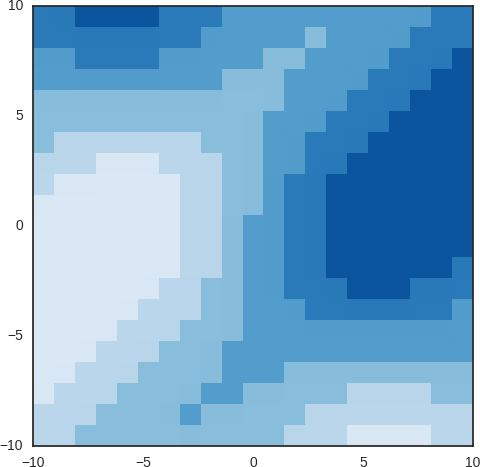
\includegraphics[height=5cm, keepaspectratio]{fig/cppn_pattern}
\caption{~}
\end{subfigure}

\caption[Example CPPN]{An example composition of the sigmoid, sinusoid and hyperbolic tangent functions.
The discrete coordinates of (b) are first normalized to $[-1.0, 1.0]$ and then mapped to various output values through the CPPN (a).
%The output pattern is visualized with different shades.
%The final neuron also has an activation function, but in this case it is the identity function, so no transformation is done.
}
\label{fig:cppn}
\end{figure}

A \textit{Compositional Pattern Producing Network} (CPPN) is an \textit{artificial development encoding} introduced by Kenneth O. Stanley in 2007 \cite{stanley-2007}.
CPPNs are structurally similar to ANNs, but differ in the use case.
Various techniques designed for ANN development and analysis may also be used for CPPNs.

Just like an ANN, a CPPN consists of a set of nodes with activation functions, weights and biases, as well as weighted connections between nodes.
Also like in an ANN, external values are input to the first layer, then undergo transformation by weights and activation functions before being outputted by the final layer.
This can be thought of as a composition of functions producing a pattern, hence the name.
An ANN is usually structured with neurons of the same activation functions,
arranged in layers,
whereas a CPPN has few such restrictions on topology and layer-wise heterogeneity.

%The difference between an ANN and a CPPN is subtle, and is primarily in the use case.
%With ANNs there is often a subset of the possible inputs that is considered "interesting" or "valid" inputs and produce interesting or valid outputs.
%With CPPNs the user is often interested in the entire mapping of all possible inputs to output and the pattern the outputs produce.
%Another difference is in the activation function of the neurons.
%In ANNs the neuron activation function is usually the same for all neurons,
%whereas in a CPPN the network consists of a variety of functions.
%The input to the network is transformed through this composition of functions.

Figure \ref{fig:cppn} shows an example CPPN and its output when mapped over a 2D Cartesian grid.
A CPPN is able to produce a pattern without multiple steps of development,
in contrast to e.g. a CA where local interactions and time is required.
CPPNs have been used both to produce patterns for the sake of the patterns, e.g. as evolutionary art \cite{stanley2006exploiting},
but also to create patterns which are used in a larger process,
such as machine learning \cite{d2008generative} and robot control \cite{risi2013confronting}.

%\subsubsection{CPPNs as CA Transition Functions}
%It is possible to use a CPPN as $\Delta$.
%The CPPN takes an $\alpha$ value as input and output a $\Sigma$ value.
%In terms of memory this CPPN $\Delta$ would not scale linearly with $K^N$.
%Because the space of possible CPPN structures is unconstrained,
%the solution space is unbounded, so some intelligent search heuristic is needed in order to find good $\Delta$ for a particular problem.


\section{Artificial Evolution and Development}
\textit{Artificial development} and \textit{artificial evolution} (evo-devo) takes inspiration from biology in order to explore large and complex solution spaces for some given problem.
% In morphogenetic engineering evo-devo is part of the third category TODO
In a typical \textit{genetic algorithm} (GA) setup \cite{holland1992genetic, mitchell-2001},
relatively simple representations of solutions are encoded as \textit{genotypes} (also called \textit{genomes}).
Through some \textit{development process} a genotype may be transformed into a \textit{phenotype} which can be used to attempt to solve the problem at hand.
The performance of the phenotype at solving the problem is the \textit{fitness} of that individual genotype.

The fitnesses of a \textit{population} of different individuals are compared.
A selection process picks individuals from the population that get to reproduce.
This selection process is usually stochastic, with a bias towards picking the individuals with the highest fitness, but some chance of picking a less fit individual now and then.
An optional part of selection can be to eliminate some fraction of the population that performed poorly, excluding them from pair selection entirely.
This is analogous to creatures in nature dying before reaching sexual maturity.
The combination of these concepts creates a \textit{selection pressure} that drives the overall population towards higher average fitness.

Individuals that are selected for reproduction are paired up.
The genotypes of the pair are combined in some fashion to create a new genotype.
In addition to the combination, random mutations may also be applied in order to produce new features not present in either parent.
As new individuals are born, the older parent generation dies out, so that the entire population is replaced.
In some cases the very best individuals of the parent generation are cloned directly into the next generation,
ensuring that their well-performing genotype continues to be present until some better genotype comes along.
This is called \textit{elitism} \cite{vasconcelos2001improvements}.

Starting out with an arbitrary initial population and repeating this generational algorithm,
it is often possible to find novel genotypes that encode good solution to the problem at hand.
Like other algorithms that search a space of solutions,
there is a risk of getting stuck in a local maximum and never finding a global maximum,
an optimal solution to the problem at hand.
There are many kinds of parameters, such as mutation rate or selection function that can be tweaked to try to avoid this.

When a phenotype is developed into a genotype, it is either possible that the genotype encodes the entire phenotype explicitly,
or it is possible that the development process augments the information stored in the genotype to create a more complex phenotype.
This is called respectively \textit{direct} and \textit{indirect encoding} \cite{clune2011performance}.
Indirect encodings allows the evolutionary search to explore a space of genotypes that is smaller than the space of possible phenotypes.
This is the way development happens in nature, where simple genomes are developed into complex lifeforms \cite{clune2011performance}.

\subsection{NEAT}
\begin{figure}
\centering
\begin{subfigure}[t]{.5\columnwidth}
\centering
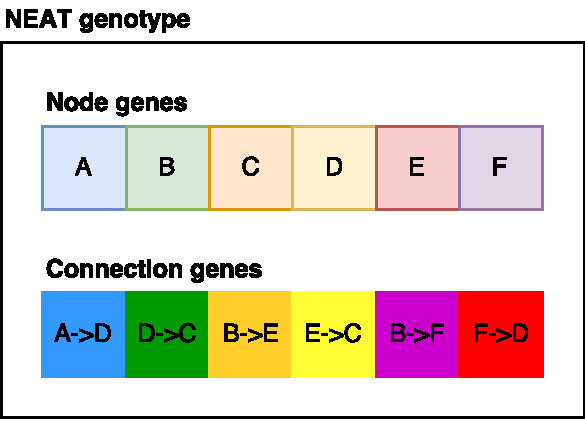
\includegraphics[height=5cm, keepaspectratio]{fig/NEAT_gt}
\caption{Genotype}
\end{subfigure}\hfill%
\begin{subfigure}[t]{.5\columnwidth}
\centering
\includegraphics[height=5cm, keepaspectratio]{fig/NEAT_pt}
\caption{Phenotype}
\end{subfigure}
\caption[Example NEAT genotype and phenotype]{
An example NEAT genotype and corresponding phenotype.
This example only shows the topology that the genotype encodes, leaving out the weights, biases and activation functions.
}
\label{fig:neat}
\end{figure}

\begin{figure}
\centering
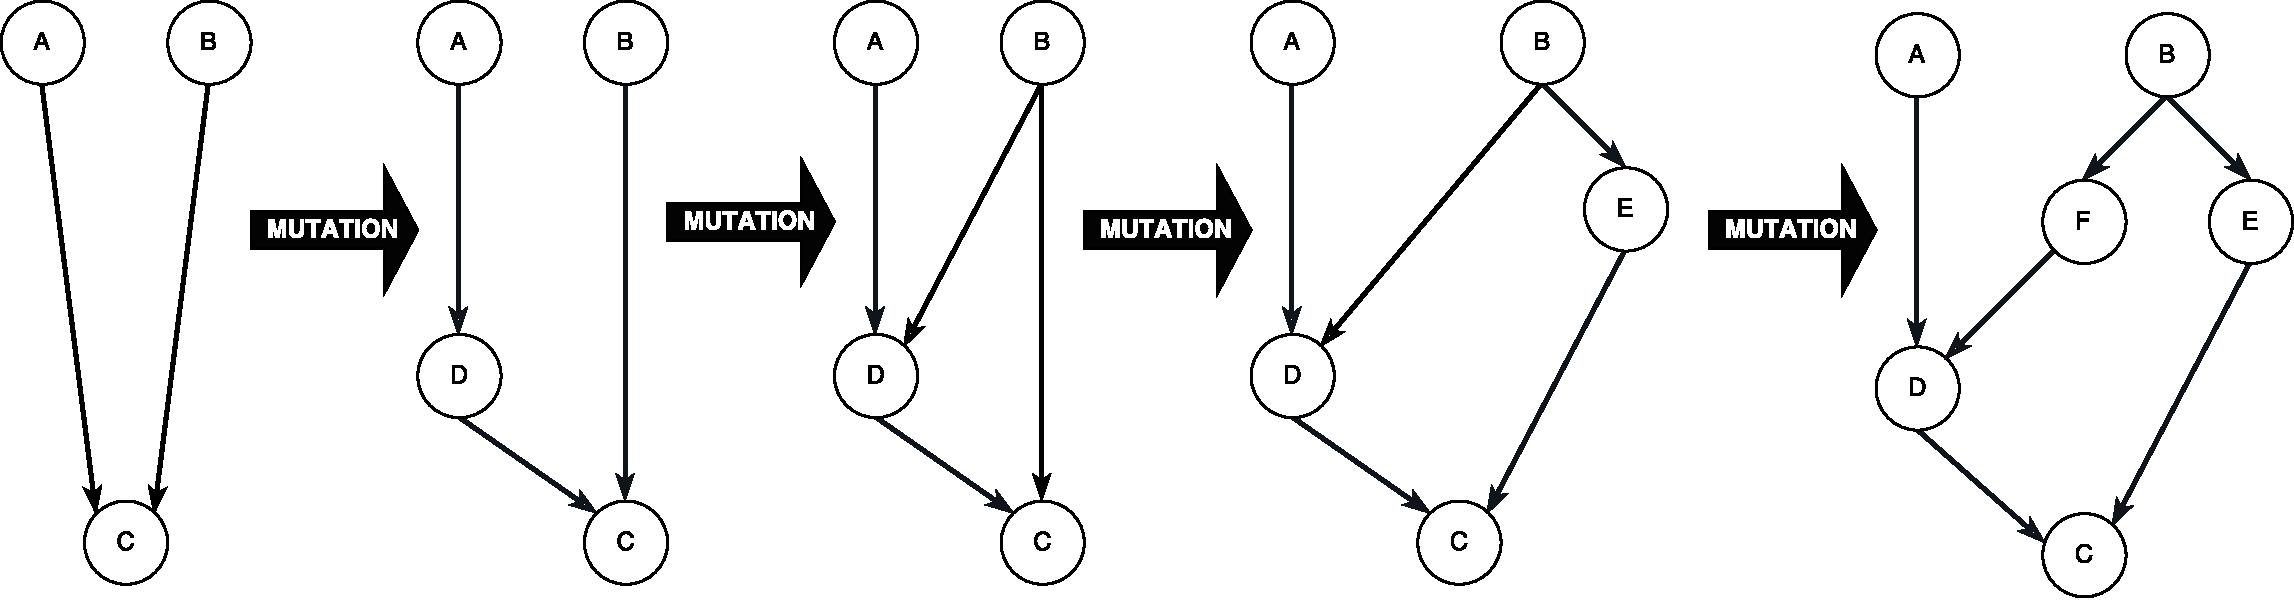
\includegraphics[width=\columnwidth, keepaspectratio]{fig/NEAT_mutation}
\caption[Example of NEAT mutation]{
    An illustrated example of NEAT mutation starting with a basic network of only two inputs and one output.
    Through the sequence, neurons and connections are added until the network is equal to that in Figure \ref{fig:neat}.
    This example shows only mutation, leaving out the crossover operation which is also part of NEAT.
    }
\label{fig:neat_mutation}
\end{figure}

\textit{NeuroEvolution of Augmenting Topologies} (NEAT) is a genetic algorithm variant introduced by Stanley and Miikkulainen in 2002 \cite{stanley-2002},
designed specifically to evolve ANNs.
When introducing CPPNs \cite{stanley-2007}, Stanley also introduced the CPPN-NEAT variation of the algorithm.

A NEAT genome consists of genes that encode nodes and connections between them.
Figure \ref{fig:neat} shows an example genotype to phenotype mapping.
NEAT starts with an initial population of very simple networks, typically with just the input and output nodes and connections between them.
Over generations, more nodes and vertices are added or disabled, activation functions are changed, and weights are adjusted.
The process of gradually expanding the genome is called \textit{complexification},
and reflects how life on earth is believed to have started with simple organisms and gradually evolved into more complex creatures \cite{darnell1986speculations,pross2005emergence}.
Figure \ref{fig:neat_mutation} shows an example of how mutation could gradually complexify a NEAT phenotype network.

The genes that make up a NEAT genome are marked with an \textit{innovation number} so that they may be recognized as the same gene in different individuals.
As new features are added to the genomes, the individuals making up the population become gradually less similar.
The degree of similarity is measured through a measure called the \textit{compatibility distance}.
When the distance between individuals pass a certain threshold, they are segregated into separate species.
This process is called \textit{speciation}.
Pair selection for reproduction happens within species.
Typically the species that have the most fit individuals will produce more children,
while the less fit species will produce fewer (but not 0) children.

When a new species appears with a new feature,
the feature will not be tuned and likely affect the fitness of the individuals negatively.
NEAT protects new species for a certain amount of time,
allowing them time to adjust before being evaluated and, if performing poorly, being extincted to make more room for the more fit species.

One notable use case of NEAT is called \textit{HyperNEAT} \cite{stanley2009hypercube}.
In this process, NEAT is used to evolve CPPNs whose output determine the topology of ANNs.
This is useful because it allows the ANN to scale easily, since the CPPN can just take more input and output more topology.
If the evolved CPPN has useful output at a small scale, it should also have a useful output at a large scale.

\subsection{Novelty Search}
\textit{Novelty search} is another genetic algorithm variant, introduced by Joel Lehmann and Kenneth O. Stanley in 2008 \cite{lehman-2008}.
It is designed to be good at \textit{deceptive} tasks, where local maximas in the fitness landscape can "deceive" conventional algorithms and prevent the search from finding the global maximum.

Novelty search avoids this by eschewing the fitness measure entirely during the search,
and instead rewards \textit{innovation}, giving higher scores to individuals that exhibit previously unseen behavior.
To find what behavior is new, an archive of seen behaviors is maintained.
A \textit{distance metric} must be selected that is appropriate for the problem at hand.
For example, if the behavior of the phenotypes produces strings, an \textit{edit distance} measure such as the \textit{Levenshtein distance} can be used.
For each genotype the $k$ nearest neighbors (in terms of behavior) are found, and the average of these distances can be used as the \textit{novelty metric}.
If a new behavior is sufficiently novel, it is added to the archive.

The algorithm is otherwise equal to NEAT, with the novelty score substituting for the objective fitness score.
This produces a population with a large variation of behaviors.
The hope is that this way, some individual "stumbles" into the global maxima.
Whether this has occurred can be determined by using the objective fitness test on the individuals of the archive.

\section{Motivation}
As mentioned in Section \ref{sec:finding_transitions},
using a more advanced encoding for CA tasks may enable a more advanced search algorithm.
This combination may then lead to successfully solving tasks that are considered difficult with the classical encoding and algorithm.

In fields such as neuroevolution,
NEAT has been shown to produce useful patterns,
without using temporal development and local interactions.
However, these tools \textit{are} used by nature in processes such as embryogenesis,
that we can model with CA.
In the quest to advance cellular systems towards biological levels of complexity,
it is worth investigating if this technique, which is proven in one field,
lends itself to being adapted as a part of a process in another field.

By testing a new model on a few select tasks, we may not only learn whether the model can accomplish the task,
but we may gain more general insights into the components (CA, the architecture; CPPN, the encoding; NEAT, the algorithm) that make up the model,
shedding further light on domains such as artificial life and morphogenetic engineering.
If something works well, we can try replacing a component with a new one to see if it still works,
or if something does not work well, we can try replacing a component to see if that changes anything.

\chapter{Related Work}
TODO rewrite and expand

In \cite{wolper-2015}, Wolper and Abraham used evolution and CPPNs to find seed patterns for Conway's Game of Life \cite{berlekamp1982winning}.
They tried both normal CPPN-NEAT (objective search) and a variation called novelty search \cite{lehman-2008}.
The results were varied, but the conclusion was in support of further research into using CPPNs for CA problems.

Many different kinds of CA encodings have been investigated previously.
These include \textit{conditionally matching rules} \cite{bidlo2013evolution, bidlo2015investigation, bidlo2015routine},
\textit{instruction-based development} \cite{bidlo2008instruction, bidlo2012evolution, nichele2016genotype,nichele2014evolutionary,nichele2016evolutionary}
\textit{self-modifying cartesian genetic programming} \cite{harding2011self}
and \textit{variable length gene regulatory networks} \cite{trefzer2013advantages}.
The paper \cite{nichele2014evolutionary} by Nichele and Tufte investigates an instruction based encoding.
The experiments in this paper repeat those of that paper, using the new CPPN encoding.



\cleardoublepage
%\chapter{Related Work}
TODO rewrite and expand

In \cite{wolper-2015}, Wolper and Abraham used evolution and CPPNs to find seed patterns for Conway's Game of Life \cite{berlekamp1982winning}.
They tried both normal CPPN-NEAT (objective search) and a variation called novelty search \cite{lehman-2008}.
The results were varied, but the conclusion was in support of further research into using CPPNs for CA problems.

Many different kinds of CA encodings have been investigated previously.
These include \textit{conditionally matching rules} \cite{bidlo2013evolution, bidlo2015investigation, bidlo2015routine},
\textit{instruction-based development} \cite{bidlo2008instruction, bidlo2012evolution, nichele2016genotype,nichele2014evolutionary,nichele2016evolutionary}
\textit{self-modifying cartesian genetic programming} \cite{harding2011self}
and \textit{variable length gene regulatory networks} \cite{trefzer2013advantages}.
The paper \cite{nichele2014evolutionary} by Nichele and Tufte investigates an instruction based encoding.
The experiments in this paper repeat those of that paper, using the new CPPN encoding.


%\cleardoublepage
%\chapter{Previous Work}
TODO

%\cleardoublepage
\chapter{Implementation}
\label{sec:implementation}

In order to conduct the experiments presented in this thesis,
a custom framework has been created in Python.
The source code is available at Github\footnote{\url{https://github.com/mathiasose/CA-NEAT/}}.
The system consists of a mix of library components and self-made components.

The CA subsystem was built from scratch.
It supports 1D and 2D grids with various border conditions (finite, toroidal, expanding), and should be easily extensible for other cases in the future.
For each problem there is a problem-specific fitness function which receives a genotype as input from the NEAT subsystem,
develops the transition function and iterates the CA  before evaluating the performance and returning a fitness value to the NEAT system.

The NEAT portion of the system is mostly based on the library \texttt{neat-python}\footnote{\url{https://github.com/CodeReclaimers/neat-python/}}.
Data structures for genomes and networks as well as various functions have been used without modifications.
The main evolutionary loop was re-implemented with modifications.
This was done for multiple reasons, including to take advantage of parallelism using \texttt{Celery}\footnote{\url{http://celeryproject.org/}} and to store the results in a database using \texttt{SQLAlchemy}\footnote{\url{http://sqlalchemy.org/}}.
Other software dependencies include \texttt{matplotlib}\footnote{\url{http://matplotlib.org/}} and \texttt{seaborn}\footnote{\url{http://seaborn.pydata.org/}} for visualization, and \texttt{dill}\footnote{\url{https://github.com/uqfoundation/dill}} for data and code serialization.

\section{CA-NEAT}
\begin{figure}
\centering
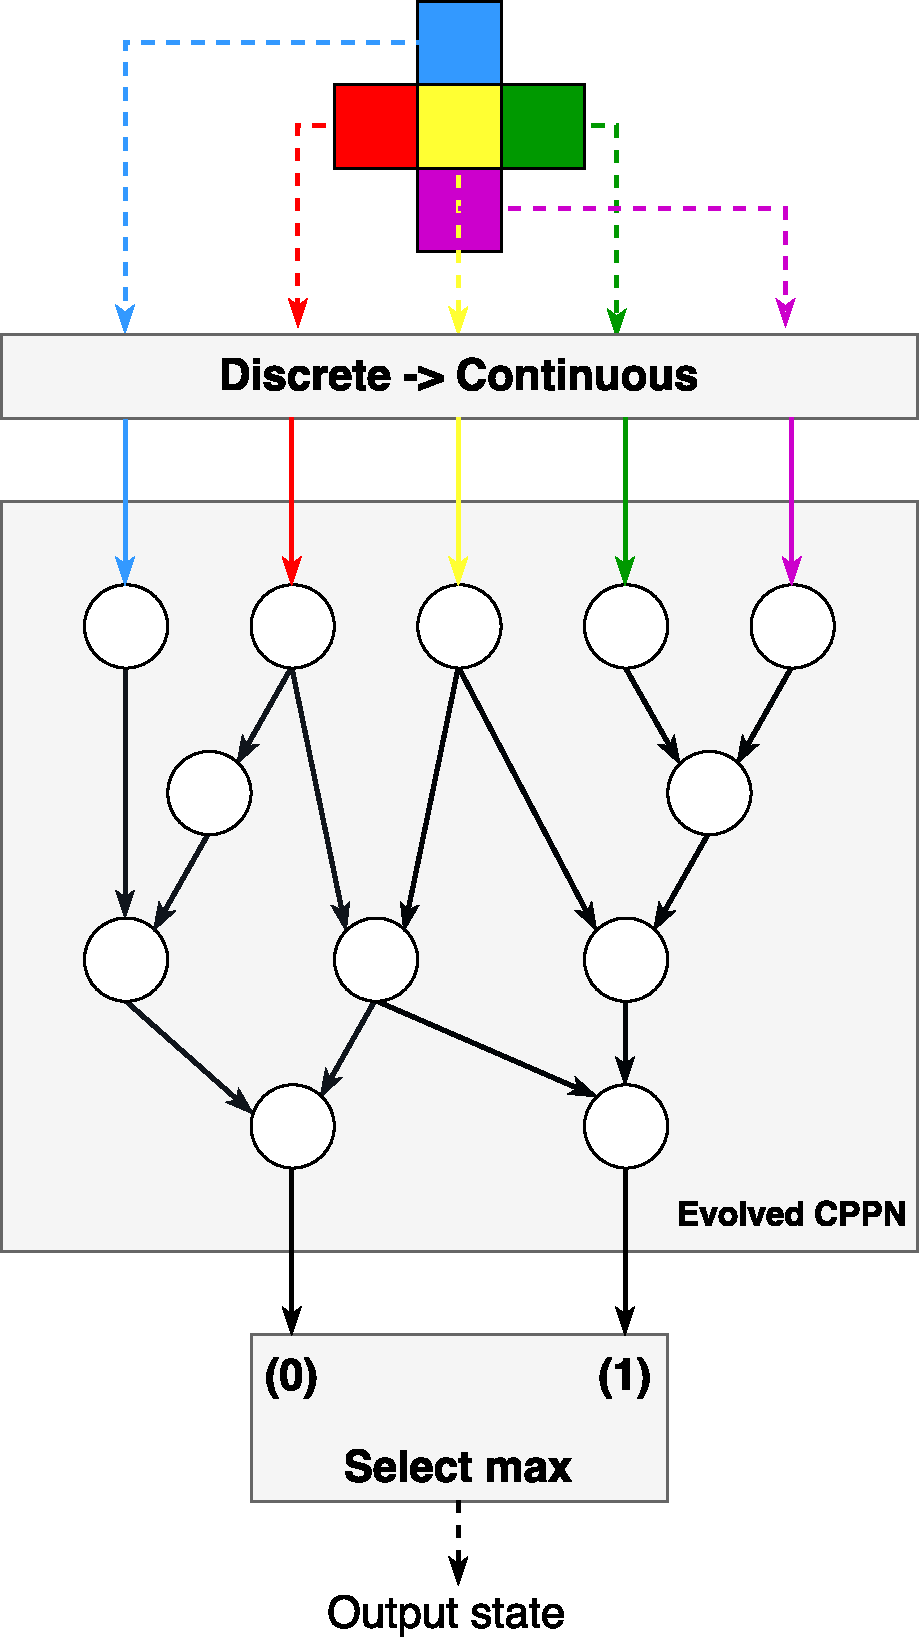
\includegraphics[width=.7\columnwidth]{fig/CA_NEAT}
\caption{
    Overview of how to use a CPPN as a CA transition rule.
    }
\label{fig:CA_NEAT}
\end{figure}

\begin{figure}
\centering
\begin{multicols}{3}
\begin{enumerate}
    \item Sigmoid
    \item Hyperbolic tangent
    \item Sinusoid
    \item Gaussian
    \item Rectified linear unit
    \item Identity
    \item Clamped
    \item Inverse
    \item Logarithmic
    \item Exponential
    \item Absolute value
    \item Hat
    \item Square
    \item Cube
\end{enumerate}
\end{multicols}
\caption{Possible activation functions}
\label{fig:activations}
\end{figure}

\begin{figure}
\centering
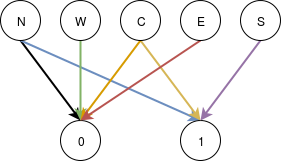
\includegraphics[width=.5\columnwidth]{fig/single_layer_cppn}
\caption
[Example first-generation CPPN with 7 out of 10 possible connections.]
{Example first-generation CPPN with 7 out of 10 possible connections. $N=5$ input nodes corresponds to the "Von Neumann" neighborhood shape, and $K=2$ output nodes correspond to a binary CA.}
\label{fig:single_layer_cppn}
\end{figure}

Since the \texttt{neat-python} library provides a NEAT implementation,
the majority of the development in this project consisted of creating the CA subsystem and the interfacing between CA code and NEAT code.

Figure \ref{fig:CA_NEAT} gives an illustrated overview of the mapping from neighborhood input to a new cell state.
The cell states are discrete values from a finite set,
but the activation functions used in the CPPN have expect inputs and outputs from the real numbers ($\mathbb{R}$).
Therefore there a mapping is performed before the CPPN input layer, assigning a continuous value to each possible cell state.
The mapping assigns each value in the finite state set to a value in the range $[-1.0, 1.0]$, evenly distanced.

The mapped values are then sent to the CPPN as input.
After the values have propagated through the network there are $K$ different outputs.
These are each paired with one of the cell states,
and the cell state corresponding to the CPPN output with the highest activation value is selected as the output and becomes the next state of the cell.

The activation functions used in the experiments in this thesis are listed in Figure \ref{fig:activations}.

The fitness evaluation function is specific to each problem.
In all experiments in this thesis, the fitness values returned are between 0 and 1, with 0 representing a complete failure and $1.0$ representing a perfectly accomplished task.

\subsection{Mapping CA-NEAT Encodings to Traditional Encodings}
\label{sec:behavior}
The mapping between the discrete and continuous number domains that happens before and after the CPPN is activated,
means that many CPPNs that are have different topologies, activation functions and weights,
will actually exhibit the exact same behavior as transition functions.
Enumerating all the possible inputs and recording the corresponding output of the transition functions creates a classical table/string representation of the transition functions.
We'll call this the \textit{behavior} of the transition function, and use this representation in analysis.

\subsection{Extending CPPN Input with Environmental Information}
\label{sec:input_extensions}
\begin{figure}
\centering
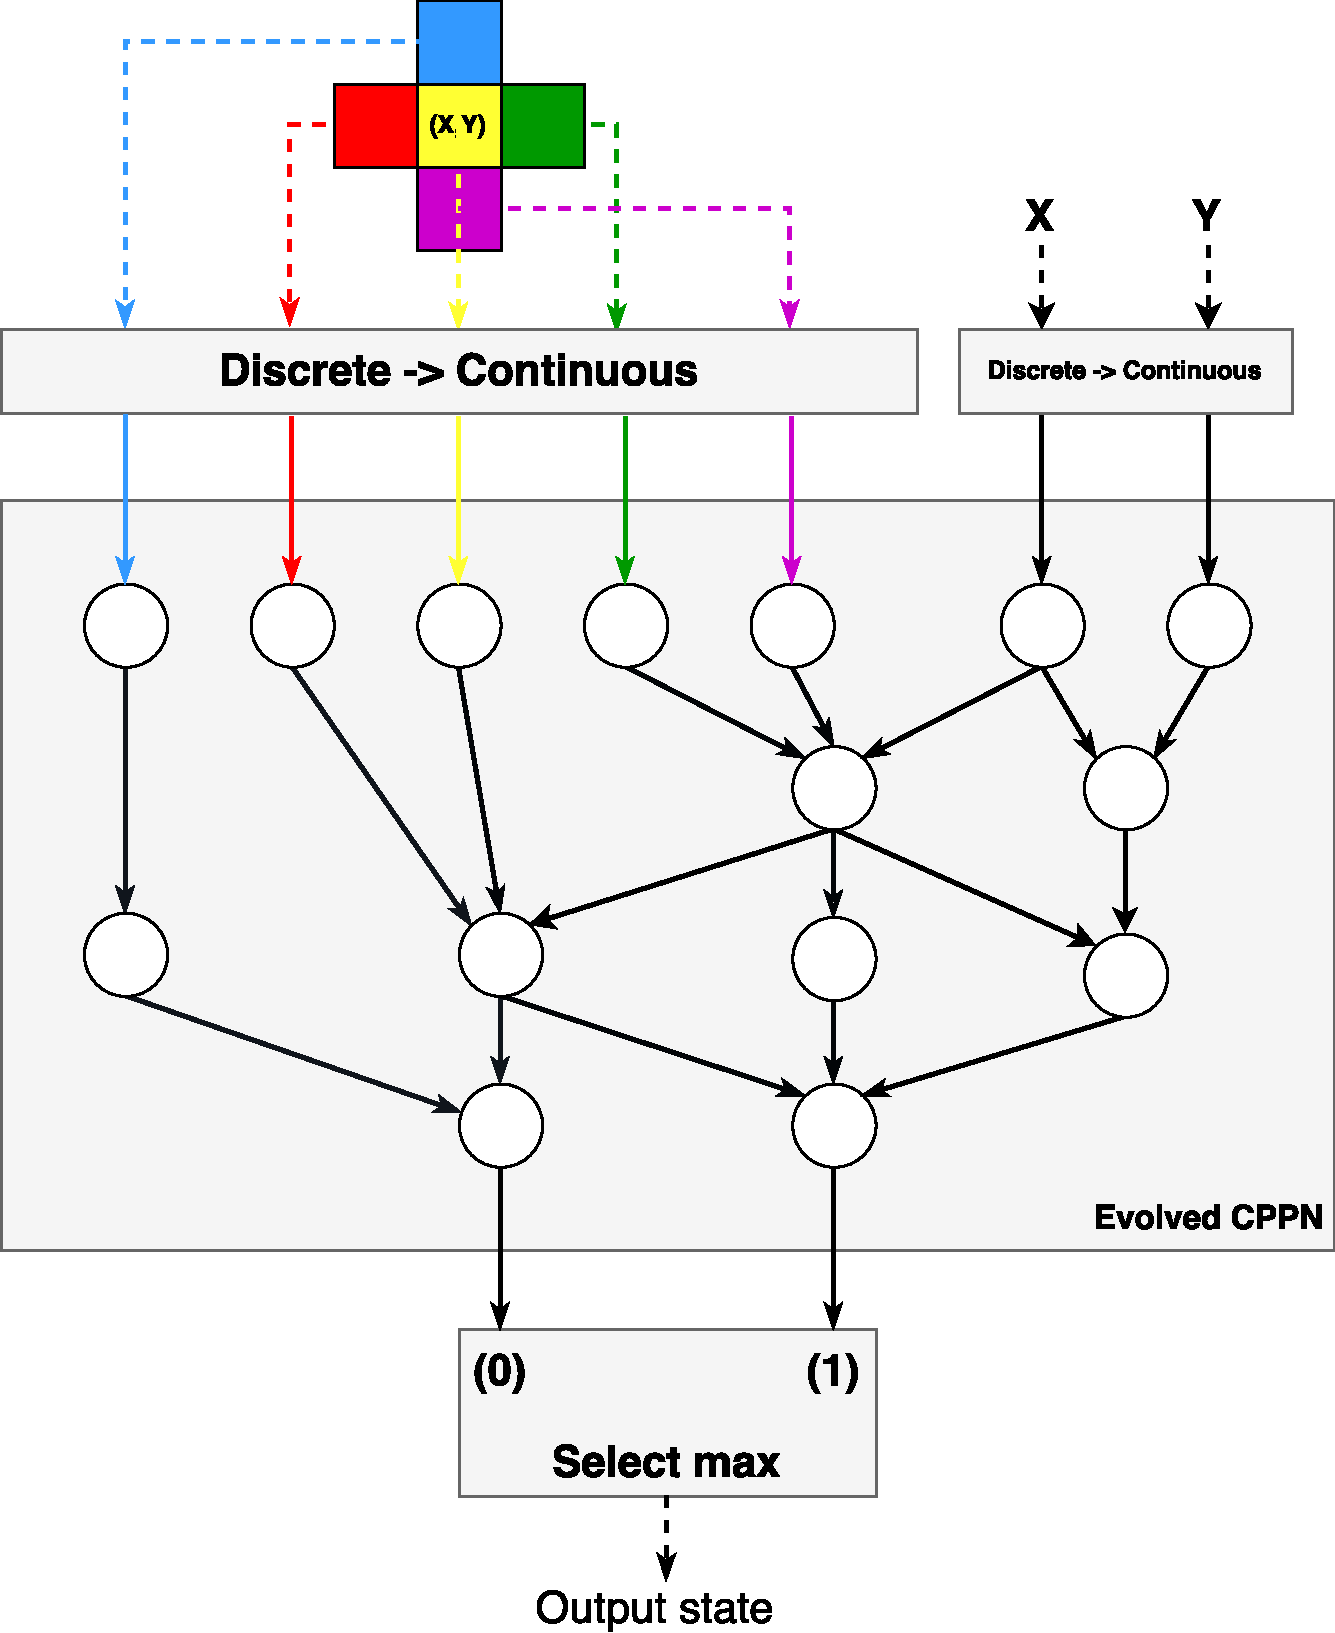
\includegraphics[width=.7\columnwidth]{fig/CA_NEAT_extension}
\caption{
    An example extension of CA-NEAT.
}
\label{fig:CA_NEAT_extension}
\end{figure}

Another aspect of CA-NEAT that can be explored, is the possibility of using inputs that are not neighboring states.
A table-based transition function is a complete mapping from all the possible inputs to a specific output.
A CPPN structure such as a CA-NEAT phenotype is less restricted in what kinds of inputs it can accept.

In biological cell systems, external factors can have large effects on the development.
For instance, a growing plant will choose which direction to expand in based on where it can find light or water in its environment.
In embryogenesis of animals,
spatial information is used to produce the correct layout of the body,
with brain cells forming in the head, skin cells on the surface of the body, and so on.
This is not all encoded in the genome of the organism, but arises from the interaction between the genome rules and the environment.

In a CA experiment, adding environmental information to the transition introduces a factor of indirect encoding,
since the same genotype can then produce different phenotypes in different environments.

Extending CA-NEAT to accept new kinds of inputs is very simple.
The NEAT part only needs to be told how many input nodes the networks should have.
Then the fitness evaluation function, which must be custom for each problem anyway,
must be programmed to extract the necessary values from the cellular model.

A concrete example is the extension used in the experiment in Section \ref{sec:morphXY}.
Figure \ref{fig:CA_NEAT_extension} illustrates this.
In addition to the neighborhood information, the coordinate values of the cell in question is also input to the network, which therefore has two additional input nodes.
The coordinate values are also mapped to the $[-1.0, 1.0]$ domain, but by a separate mapping function.

\section{Novelty Search}
\label{sec:novelty}
Novelty search has been added in as an extension to the existing CA-NEAT framework.
Many CA problems can be "deceptive" to a GA and to the programmer tasked with creating an appropriate fitness function.
The CA must transition through a sequence of intermediate states before arriving at the desired target state,
but it is not necessarily clear what intermediate behavior should be rewarded in order to find the final result.
This makes a good case for testing novelty search for these problems.

In order to extend CA-NEAT for novelty search, some phenotype value needs to be measured and compared in order to calculate novelty.
The enumerated "string" representation of the transition function was selected for this.
The \textit{Hamming distance} between different strings can then be calculated and used as a measure of novelty distance.
The distances are normalized to the $[0.0, 1.0]$ range and the mean of the $k=15$ closest distances is used for the innovation score of the individuals.
The threshold for adding a genotype to the innovation archive is initialized at $0.5$, but is dynamically adjusted throughout the run.
If $0$ genotypes are added in a generation, the algorithm will pick one at random to add anyway, and also decrease the threshold by multiplying with a factor between $0.95$ and $1.0$.
If more than $5$ individuals are added in a generation, they will all be added, and afterwards the threshold is increased by multiplying with a factor between $1.0$ and $1.05$.
The adjusting factors are picked at random from a uniform distribution.
This should allow the threshold to eventually settle into an appropriate value, and the randomness should prevent it from oscillating between two different values.


\cleardoublepage
\chapter{Experiments}
\label{chap:methodology}
\label{chap:experiments}

\section{Overarching Methodology}
Several of the following sections are about selecting a CA problem and letting CA-NEAT have a go at solving it.
In these experiments, the same basic configuration of CA-NEAT is used.
The size of the CA neighborhood (equal to the number of CPPN inputs) and the number of cell-states (equal to the number of CPPN outputs) is changed to be appropriate to the problem at hand.
The fitness evaluation function is also custom to every problem.

Otherwise the CA-NEAT parameters are the same across different experiments.
These are listed in Appendix TODO.
%Notably, the mutation weigths are biased towards adding nodes and connections moreso than removing them, leading to the average network size growing over time.

Each experiment consists of 100 independent runs with the same parameters but different initial populations.
All experiments have a population size of 200 individuals and elitism degree of 1.
Each generation-population is segregated into species by NEAT, with selection and reproduction happening within these groups.
\textit{Sigma scaled selection} \cite{hancock-1994} is used to select pairs for reproduction.

During development of the system, a variation of different configurations were tried for different problems.
When deciding on the experiments to collect results from for this paper,
a deliberate choice was made to use the same CPPN-NEAT configuration and as close to the same CA configuration as possible for all problems.
This makes it easier to make comparison between experiments, but means that the settings chosen may favor some experiments over others.

\section{Morphogenesis and Replication of 2D Patterns}
\label{sec:prev_work}
The first class of problems CA-NEAT was tested on was \textit{morphology problems}, in the form of the two related problem of morphogenesis and replication.
The patterns used in these experiments are shown in Figure \ref{fig:patterns}

\begin{figure*}
\centering
\begin{subfigure}[b]{.20\textwidth}
\centering
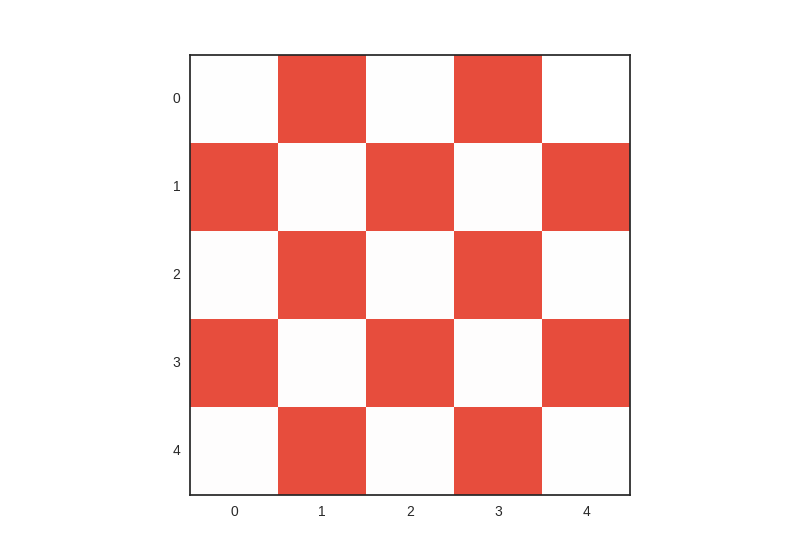
\includegraphics[width=\textwidth]{fig/mosaic}
\caption{5x5 "Mosaic"}
\label{fig:mosaic_pattern}
\end{subfigure}%
\begin{subfigure}[b]{.20\textwidth}
\centering
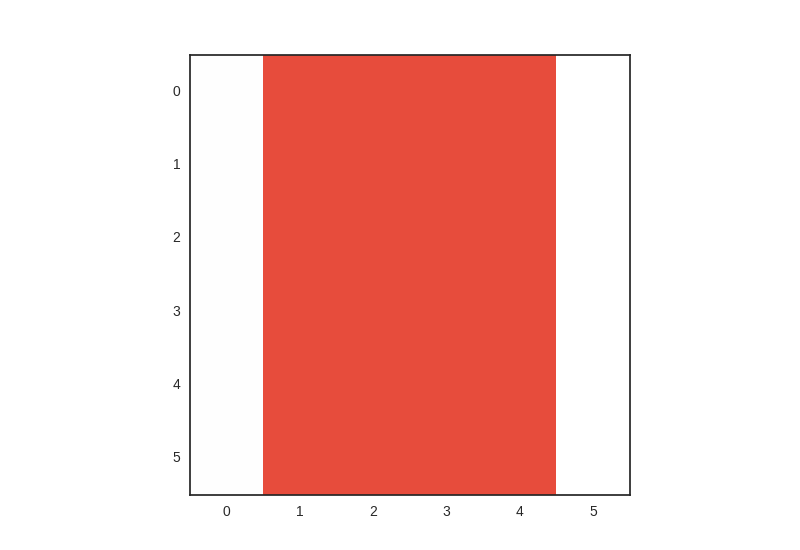
\includegraphics[width=\textwidth]{fig/border}
\caption{6x6 "Border"}
\end{subfigure}%
\begin{subfigure}[b]{.20\textwidth}
\centering
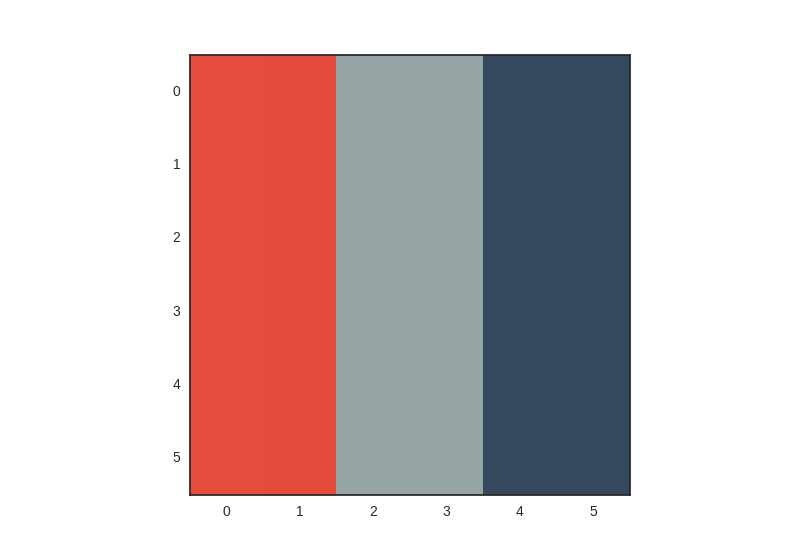
\includegraphics[width=\textwidth]{fig/tricolor}
\caption{6x6 "Tricolor"}
\end{subfigure}%
\begin{subfigure}[b]{.20\textwidth}
\centering
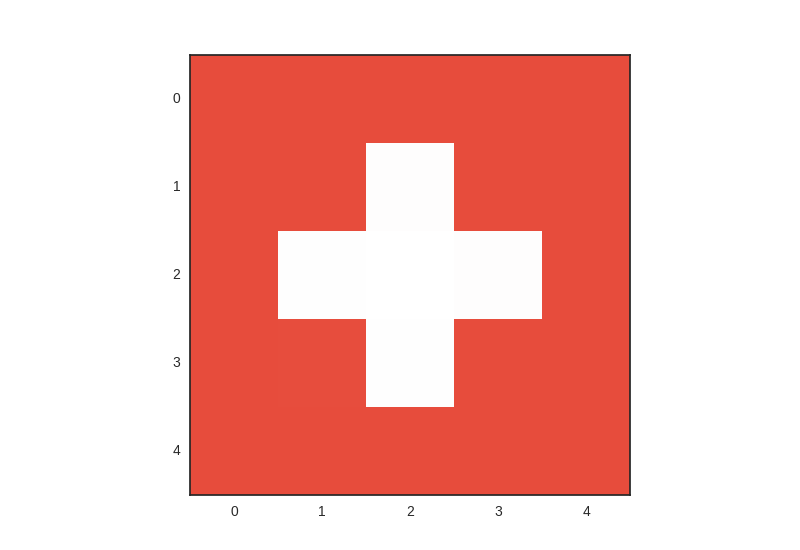
\includegraphics[width=\textwidth]{fig/swiss}
\caption{5x5 "Swiss"}
\end{subfigure}%
\begin{subfigure}[b]{.20\textwidth}
\centering
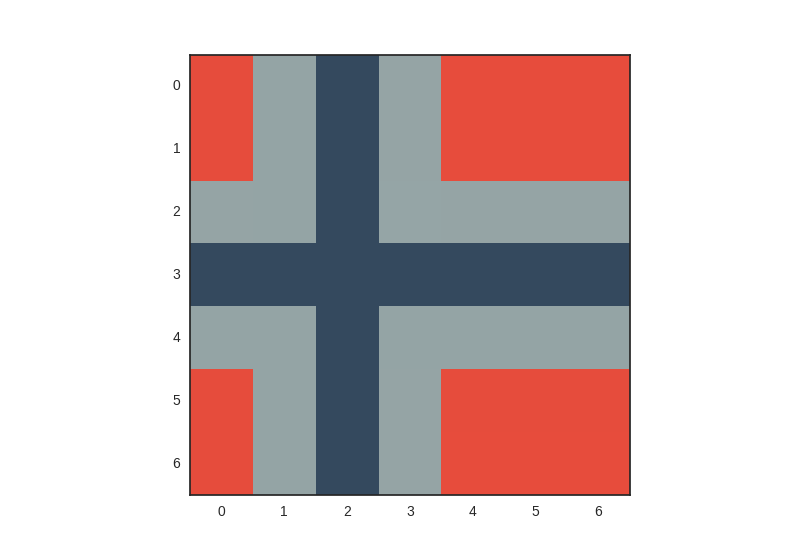
\includegraphics[width=\textwidth]{fig/nordic}
\caption{7x7 "Nordic"}
\end{subfigure}%

\caption{Patterns being investigated for morphogenesis and replication.}
\label{fig:patterns}
\end{figure*}

These are the same problems and patterns as studied in \cite{nichele2014evolutionary}, which used an instruction-based encoding and also tested table-based encoding for comparison.
This allowed the results of \cite{nichele2014evolutionary} to act as a benchmark for testing the CA-NEAT framework during development,
and to make comparisons between the results for analysis.

The experiments in this section were performed and analyzed in the specialization project leading up to this thesis project.
The report from the specialization project was further refined with co-authors Stefano Nichele, Gunnar Tufte and Sebastian Risi to a paper which at the time of writing has been accepted but not yet published in the IEEE Transactions on Cognitive and Developmental Systems.
TODO does mentioning the above go somewhere else?

\subsection{Morphogenesis problems}
\label{sec:morph_problems}
In CA terms, morphogenesis is the construction of a (more) complex pattern from a simple "seed" pattern.
The biological analogy and inspiration is \textit{embryonic development},
with the seed pattern also sometimes called a \textit{zygote}.
Figure \ref{fig:seed} shows the seed patterns used in these experiments.

\begin{figure}
\centering
\begin{subfigure}[b]{.30\columnwidth}
\centering
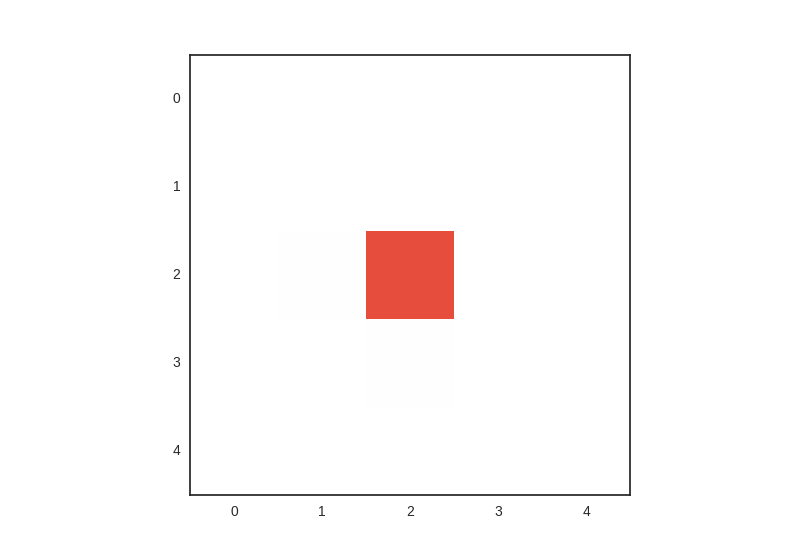
\includegraphics[width=\columnwidth]{fig/seed_5x5}
\caption{5x5}
\end{subfigure}%
\begin{subfigure}[b]{.30\columnwidth}
\centering
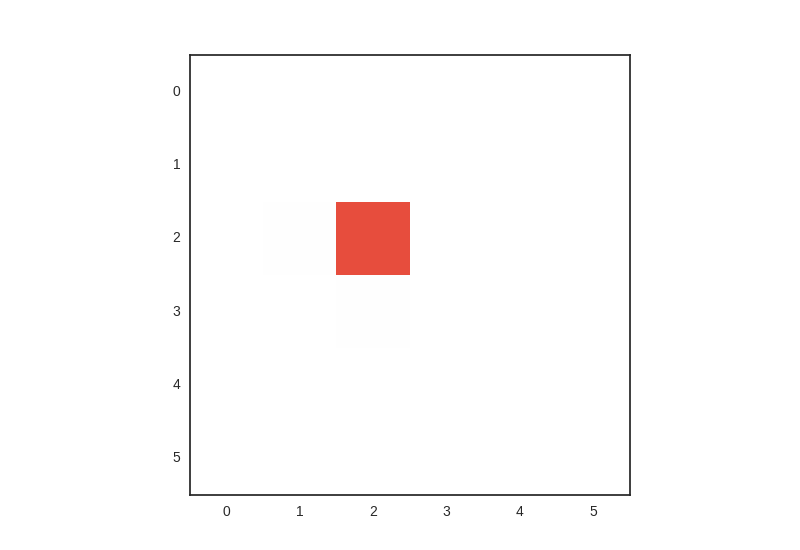
\includegraphics[width=\columnwidth]{fig/seed_6x6}
\caption{6x6}
\end{subfigure}%
\begin{subfigure}[b]{.30\columnwidth}
\centering
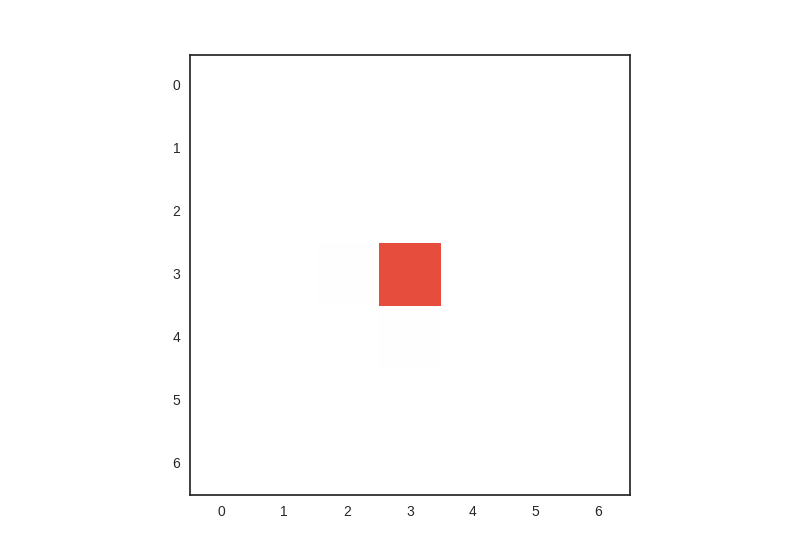
\includegraphics[width=\columnwidth]{fig/seed_7x7}
\caption{7x7}
\end{subfigure}%

\caption
[
    Seed patterns for morphogenesis.
]
{
    Seed patterns for morphogenesis.
    For the 6x6 patterns there is no central cell, so the seed is not symmetric.}
\label{fig:seed}
\end{figure}

The fitness evaluation function used in the morphogenesis experiments consists of the following steps:

\begin{enumerate}
    \item Develop seed pattern for 30 iterations
    \item For each stage
        \begin{enumerate}
            \item Compare cell by cell with  target pattern
            \item Calculate ratio of correct out of total cells
        \end{enumerate}
    \item Pick the highest of the values from step 2
    \item Use function \eqref{eq:redistribute} with value from step 3 as x
\end{enumerate}

\begin{equation}
    \label{eq:redistribute}
    f(x) = x * \frac{e^{5*x}}{e^{5}}
\end{equation}

In cases such as the "Mosaic" pattern (Figure \ref{fig:mosaic_pattern}), a completely dead CA (all cells in the quiescent state) would have a "correct cell" ratio of $0.52$.
Function \eqref{eq:redistribute} is used to reduce the score for such cases, while ensuring that $f(1.0) = 1.0$.

Because every iteration of the CA is counted equally and separately,
the fitness evaluation does not care if the CA becomes stable, enters a cycle, or neither within the 30 allotted iterations.
If the target pattern occurs at any point, that is enough to get a perfect score.

\subsection{Replication problems}
In a CA replication problem, the initial state has some complex pattern present.
The goal is to produce multiple copies of this initial patterns within the allotted time.
The biological analogy of this is cell division and asexual (clonal) reproduction.
For the replication problem the seed pattern is thus one copy of the target pattern in a larger grid.

The fitness evaluation for a replication phenotype is as follows:

\begin{enumerate}
    \item Develop seed pattern for 30 iterations
    \item For each stage
        \begin{enumerate}
            \item For each region of target pattern size
            \begin{enumerate}
                \item Compare cell by cell with  target pattern
                \item Calculate ratio of correct out of total cells
            \end{enumerate}
            \item Pick the highest 3 values from (a)
            \item Multiply any value less than $1.0$ by a penalty factor of $0.9$
            \item Calculate mean of three values
        \end{enumerate}
    \item Pick the highest value from stage (2)
\end{enumerate}

In this case the number of replicas sought is three.
There is no further contribution to the score if there are more than three perfect replicas.
But it follows logically that if one instance can be duplicated once, then each of the duplicates should be able to duplicate again, leading to exponential growth if time and space is not bounded.
Once again a penalty is applied, this time to penalize the contribution from any imperfect replica pattern, hopefully driving the selection pressure towards perfect replication.

Compared to the evaluation of morphogenesis of the same pattern, the replication evaluation is much more computationally expensive.
Therefore it will always take longer to collect results for a replication problem than the same-pattern morphogenesis problem.

\subsection{Cellular Model}
For both morphology problem categories a 2D CA model is used.
For the morphogenesis problem the grid is of fixed size with toroidal border conditions.
For the replication problem the grid is automatically expanding to accommodate growth in any direction.
In theory this means an infinite grid, but since the CA may only iterate 30 times, there is a practical limit to how large it may grow.
For both problem types the Von Neumann neighborhood (Figure \ref{fig:neighborhoods_vn}) is used.

\subsection{Results}
\begin{table*}[h]
    \centering
    \caption[Summary of results of morphology experiments]{
Summary of results.
The metrics shown are the success rate and the mean number of generations until a solution is found, with standard deviation also shown.
In the case of 100\% success rate, the number of generations column shows how many generations it took until the final solution was found.
In the case of less than 100\% success rate, the column shows how many generations were run until the experiment was stopped.
}
\begin{tabular}{lrrrr}
\hline
 Problem              &   Success rate \% &   Mean gens. &   $\sigma$ gens. &   Gens. until stop \\
\hline
Mosaic morphogenesis      &              100 &                1.2 &                 0.4 &                        2 \\
Border morphogenesis      &                1 &              270   &                 0   &                      509 \\
Tricolor morphogenesis    &              100 &               56.5 &               228.8 &                     2189 \\
Swiss morphogenesis       &               76 &              147.7 &               158.9 &                      600 \\
Mosaic replication        &              100 &                4.2 &                10.6 &                       99 \\
Swiss replication         &              100 &                7.7 &                 5   &                       20 \\
Tricolor replication      &               55 &               55.8 &                52.6 &                      200 \\
Nordic replication        &               0  &                  - &                   - &                      200 \\
\hline
\end{tabular}
\label{tbl:results}
\end{table*}

\begin{table}
    \centering
    \caption{Success rate at morphology problems for table-based, instruction-based and CA-NEAT transition functions found by GA.}
    \begin{tabular}{llll}
    \hline
    Problem                & Table-based & Instruction-based & CA-NEAT \\ \hline
    Mosaic morphogenesis   & 55\%        & 98\%              & 100\%   \\
    Swiss morphogenesis    & 23\%        & 100\%             & 76\%    \\
    Border morphogenesis   & 69\%        & 98\%              & 1\%     \\
    Tricolor morphogenesis & 19\%        & 46\%              & 100\%   \\
    Mosaic replication     & 85\%        & 100\%             & 100\%   \\
    Swiss replication      & 1\%         & 100\%             & 100\%   \\
    Tricolor replication   & 8\%         & 100\%             & 45\%    \\
    Nordic replication     & 0\%         & 100\%             & 0\%     \\ \hline
    \end{tabular}
\end{table}

\begin{figure}[t]
\centering
\begin{subfigure}[t]{.45\columnwidth}
\centering
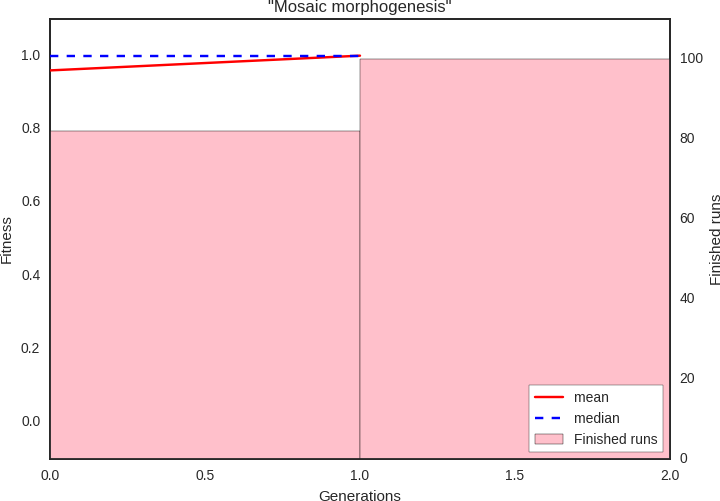
\includegraphics[width=\columnwidth]{fig/generate_mosaic_results}
\caption{Mosaic pattern morphogenesis, all generations.}
\label{fig:generate_mosaic_results}
\end{subfigure}
\begin{subfigure}[t]{.45\columnwidth}
\centering
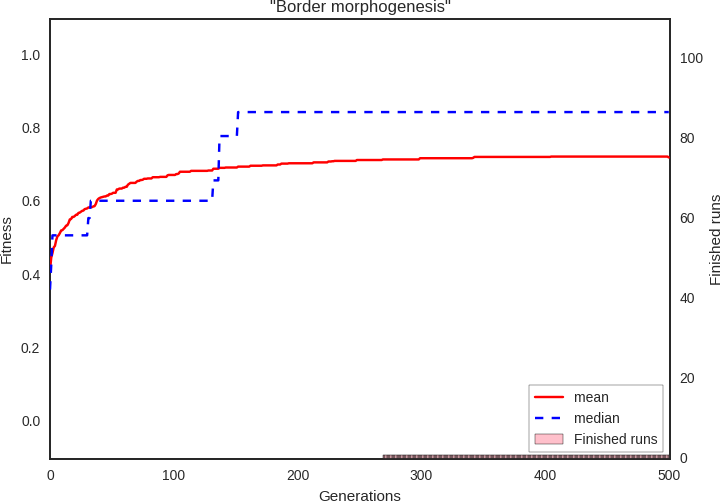
\includegraphics[width=\columnwidth]{fig/generate_border_results}
\caption{Border pattern morphogenesis, 500 first generations.
%The value where the median stabilizes represents the fitness for a solution with one wrong cell.
}
\label{fig:generate_border_results}
\end{subfigure}
\begin{subfigure}[t]{.45\columnwidth}
\centering
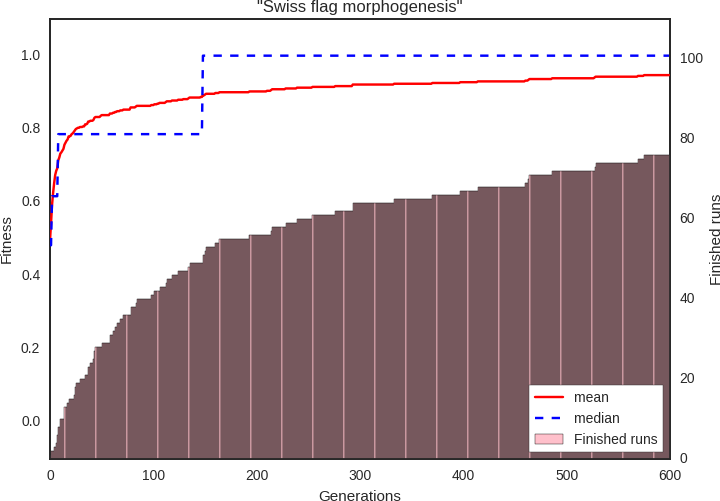
\includegraphics[width=\columnwidth]{fig/generate_swiss_results}
\caption{Swiss flag pattern morphogenesis, 600 first generations.}
\label{fig:generate_swiss_results}
\end{subfigure}
\begin{subfigure}[t]{.45\columnwidth}
\centering
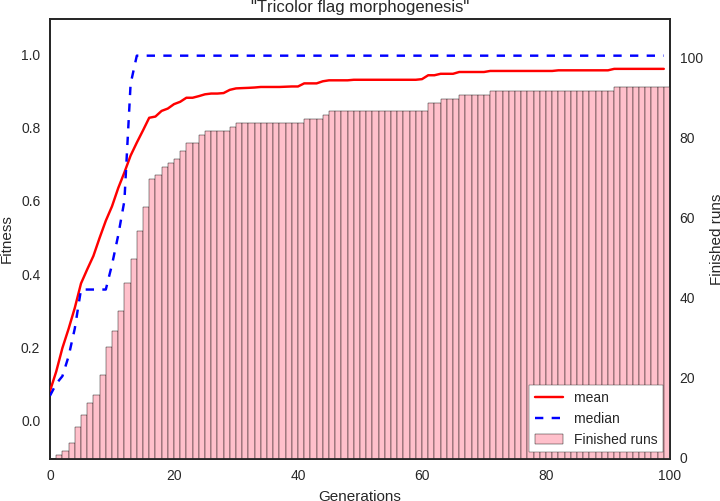
\includegraphics[width=\columnwidth]{fig/generate_tricolor_results}
\caption{Tricolor flag pattern morphogenesis, 100 first generations.}
\label{fig:generate_tricolor_results}
\end{subfigure}
\caption{
    Success rate (cumulative histogram) of the morphogenesis experiments.
    Also shows the mean and median of the max fitness in each run.
    }
\label{fig:morphogenesis_results}
\end{figure}

\begin{figure}[t]
\centering
\begin{subfigure}[t]{.45\columnwidth}
\centering
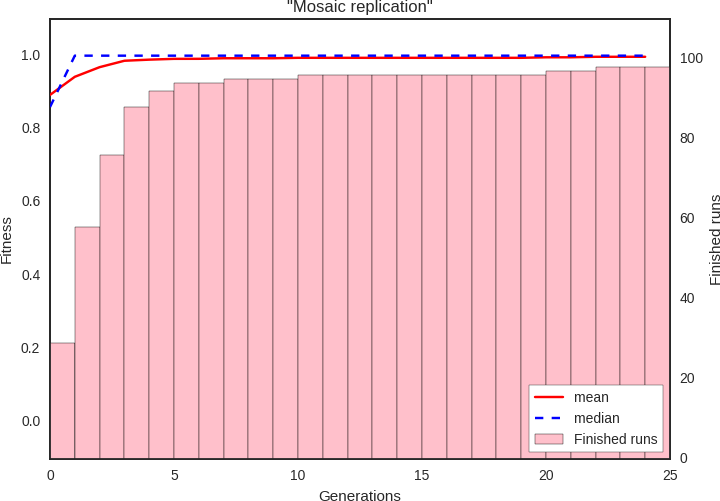
\includegraphics[width=\columnwidth]{fig/replicate_mosaic_results}
\caption{Mosaic pattern replication, 25 first generations.}
\label{fig:replicate_mosaic_results}
\end{subfigure}
\begin{subfigure}[t]{.45\columnwidth}
\centering
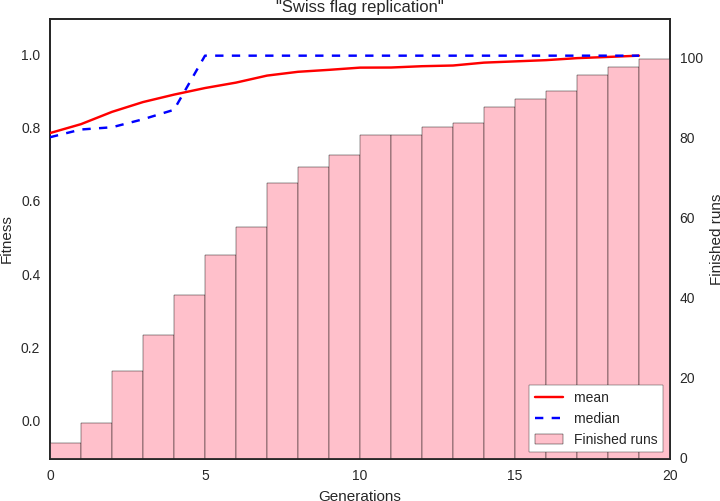
\includegraphics[width=\columnwidth]{fig/replicate_swiss_results}
\caption{Swiss flag pattern replication, all generations.}
\label{fig:replicate_swiss_results}
\end{subfigure}
\begin{subfigure}[t]{.45\columnwidth}
\centering
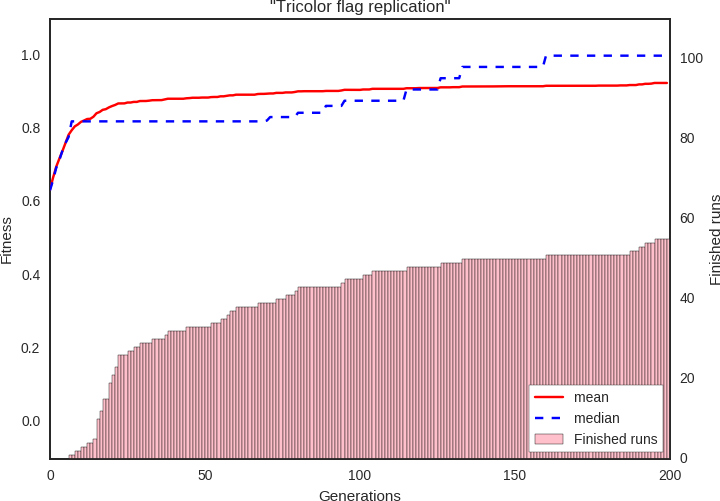
\includegraphics[width=\columnwidth]{fig/replicate_tricolor_results}
\caption{Tricolor flag pattern replication, 200 first generations.}
\label{fig:replicate_tricolor_results}
\end{subfigure}
\begin{subfigure}[t]{.45\columnwidth}
\centering
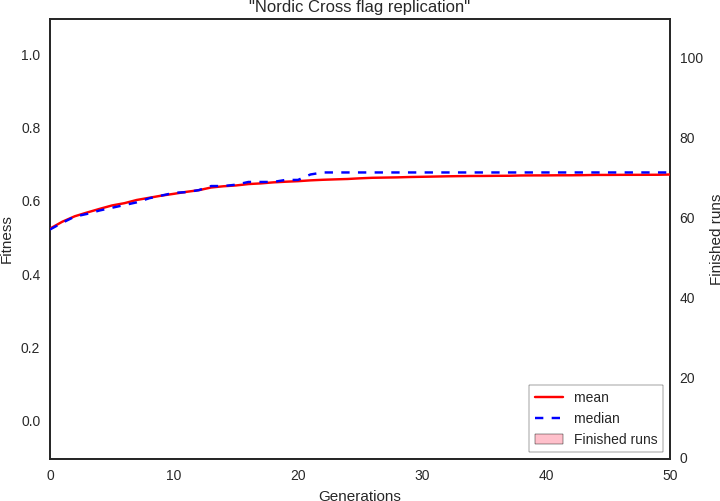
\includegraphics[width=\columnwidth]{fig/replicate_nordic_results}
\caption{Nordic cross pattern replication, 50 first generations.
%Further generations up to 200 did not have any significant change in the mean or median lines.
}
\label{fig:replicate_nordic_results}
\end{subfigure}
\caption{TODO}
\label{fig:replication_results}
\end{figure}

The results of the experiments were varied, with some problems being easily solved with CA-NEAT, some being slowly solved, and some not being consistently solved at all.
Table \ref{tbl:results} summarizes the results in terms of success rate and generations of evolution.
In addition to the varied success rate, there was also a large variation in how many generations of evolution was required to find solutions.
In many cases there was at least one optimal solution among the 20000 individuals generated as part of initial populations.
This means there exists a simple solution consisting of only the input and output layers with connections. 
The most extreme of these cases is the ”Mosaic” morphogenesis where 80 runs complete in the initial generation and the last 20 in the second generation.
This result is understandable, since the pattern has so much symmetry and repetitiveness.
For more complex patterns, more generations of evolution is required in order to bring the success rate nearer 100\%.

It is somewhat surprising which problems are easily solved and which ones are difficult.
The "Swiss" replication is much easier than the "Swiss" morphogenesis,
but the "Tricolor" morphogenesis is easier than the replication of the same pattern.
The fact that the "Border" morphogenesis is much more difficult than the "Tricolor" morphogenesis is not intuitive,
since the "Border" pattern has both fewer colors and one more symmetry.
%Figure \ref{fig:border_almost_correct} shows an example of the close but not perfect patterns CA-NEAT produces for the "Border" morphogenesis.
Perhaps it is the symmetry that is the "trap" which leads to a local maxima,
and the "Tricolor" experiment avoids this,
since symmetry in solutions will not give great scores in that case.
Since the other morphogenesis experiments succeed, and one "Border" solution is found,
there is little reason to suspect that there is any technical error causing poor results.
So the reason must be that the combination of algorithms, problem and parameters cause the problem to be very difficult.
%Further work is required to investigate this.

CA-NEAT does quite well for three out of four replication problems, but fails completely at the "Nordic" replication.
This problem can be expected to be quite difficult, since the pattern is rather complex.
But the instruction-based encoding in \cite{nichele2014evolutionary} did well at the task,
so it is certainly possible to solve the problem with this particular cellular model.
The development of the mean and median lines shown in Figure \ref{fig:replicate_nordic_results} indicate that the evolutionary searches find local maxima from which they can't escape.
%This, along with the "Border" morphogenesis results,
%suggest that the search heuristic may be unsuitable for these problems, and should be reconsidered.

These results were compared with the results of \cite{nichele2014evolutionary}.
It was found that CA-NEAT was able to significantly outperform instruction- and table-based encodings at some problems, while also performing much worse at other problems.
At the morphogenesis tasks, CA-NEAT outperformed the table-based evolution at 3/4 tasks and the instruction-based evolution at 2/4 tasks.
For the replication tasks, CA-NEAT outperformed the table-based evolution at 3/4 tasks and tied at 0\% for the last task.
Instruction-based evolution had a 100\% success rate at all replication tasks.
CA-NEAT equaled this rate at two of the tasks, had some success at one task, and failed completely at the last task.

Figures \ref{fig:tricolor_point_attractor} and \ref{fig:mosaic7} shows visualizations of two results found by evolution.
A larger selection of visualizations is available in the appendix of TODO.

TODO

\begin{figure}
\centering
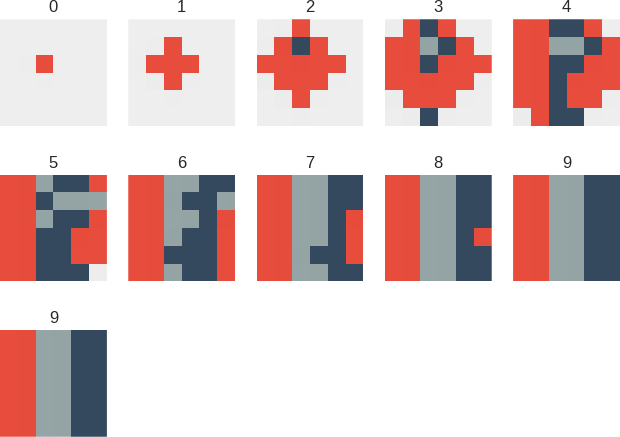
\includegraphics[width=\textwidth, keepaspectratio]{fig/result_figs/generate_tricolor/1}
\caption[A solution to the "Tricolor" morphogenesis]{A solution to the "Tricolor" morphogenesis that finds a point attractor equal to the target pattern.
Most solutions seen did not stabilize like this, but instead found a variety of cycles.}
\label{fig:tricolor_point_attractor}
\end{figure}

\begin{figure}
\centering
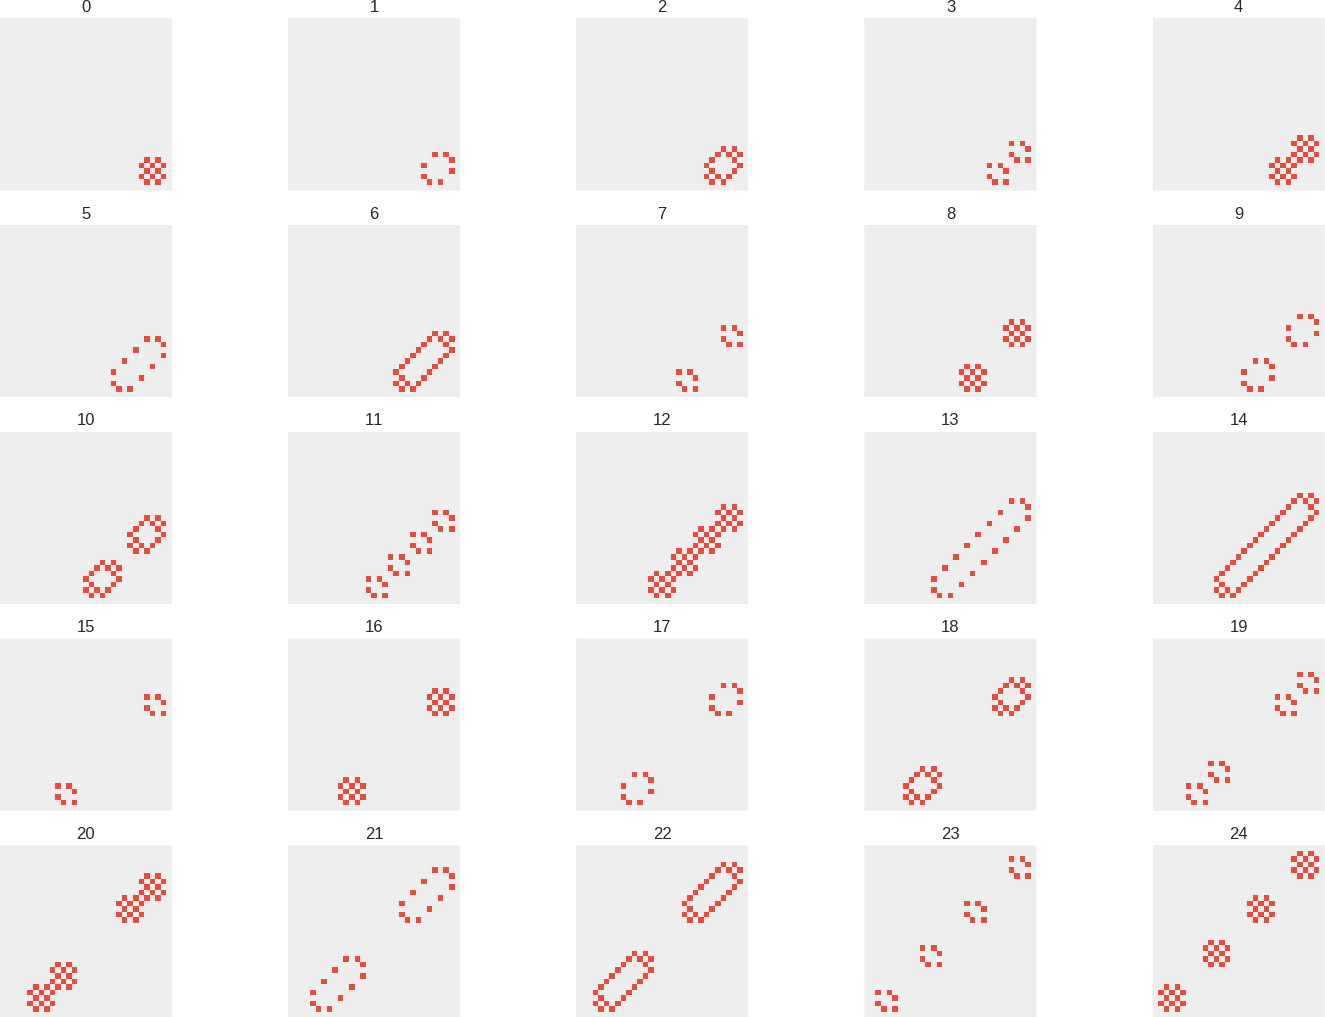
\includegraphics[width=\textwidth, keepaspectratio]{fig/result_figs/replicate_mosaic/7}
\caption[A solution to the "Mosaic" replication]{A solution to the "Mosaic" replication that shows multiple stages of replication.
First the original replicates into two copies. Then each copy tries to replicate, but they interfere with each other and instead return to one copy each, but at a greater distance.
Then they each succeed in replicating, producing four copies total.}
\label{fig:mosaic7}
\end{figure}


\section{2D Morphogenesis With Coordinate Inputs}
\label{sec:morphXY}
Adding environmental information to the CA may make it possible to solve a task that is difficult with only the neighborhood information.
The morphogenesis task makes for a nice test case.
For this experiment, the cellular model is extended to include coordinate information, as described in Section \ref{sec:input_extensions}.
The "Border" and "Nordic" patterns (Figure \ref{fig:patterns}) are targeted in separate experiments.
The "Border" morphogenesis in the previous experiment did not work very well, so it makes for a good comparison.
The "Nordic" pattern is also difficult to generate with the cellular model (TODO because), so it was not attempted in the previous experiment,
but is attempted now.

The quiescent rule is still in place: a cell may not change state if all the neighbors are quiescent, even if the information from the coordinates is available to inform a decision.
The coordinate information is meant to be used in conjunction with the neighborhood information, not to replace it.
If this was not the case, evolution could come up with a CPPN where all the neighborhood inputs were disconnected from the output,
and a static pattern was produced in one time step, like in Figure \ref{fig:cppn}.
That is not a result that we are interested in.

\subsection{Results}

\begin{figure}
\centering
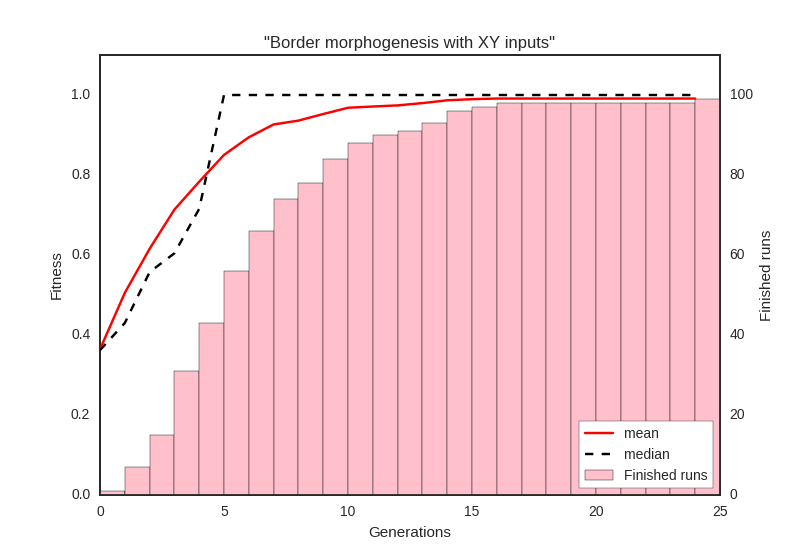
\includegraphics[width=\textwidth, keepaspectratio]{fig/generate_border_extended_results}
\caption{
    TODO
    One trial had yet to succeed when the experiment was stopped at 100 generations.
}
\label{fig:generate_border_extended_result}
\end{figure}


\begin{figure}
\centering
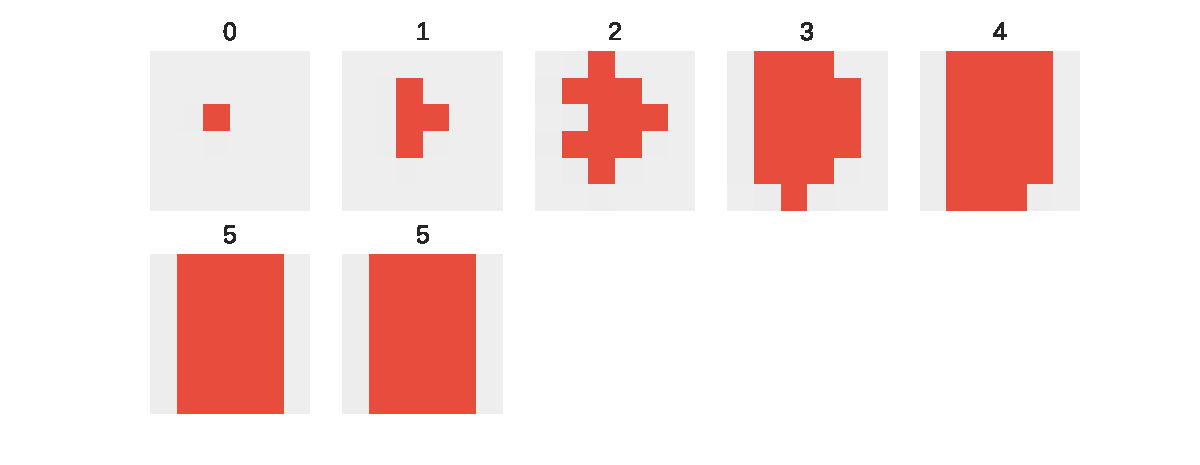
\includegraphics[width=\textwidth, keepaspectratio]{fig/result_figs/border_point_5}
\caption{
    TODO
}
\label{fig:border_point_5}
\end{figure}

TODO

\section{Majority Problem}
The \textit{majority problem} is a problem for 1D binary CA.
It is also called the \textit{density classification task} in literature \cite{mitchell1993revisiting, mitchell1996evolving}.
In this task, the CA should have some arbitrary initial configuration where one "color" (black/white) is more common than the other.
The CA must then figure out which color this is and end up in a point attractor state where all the cells are of this color.
Depending on the initial configuration this can be easy, or very difficult, so finding a general solution that can figure out any initial configuration is difficult.
Even if the majority of the configuration is black, there might be a sub-region that is majority white.
The lack of global overview means that the CA needs to send information around the grid and "negotiate" a consensus about the color.
This problem has been studied extensively with table-based transition functions found by genetic algorithm \cite{mitchell1993revisiting, mitchell1996evolving, mitchell-2001} 

The experiment design here is inspired by the design in TODO cite.

10 initial configurations are created with a specific ratio of black and white cells, but in a random order.
Five are white-dominated and five are black-dominated.
The fitness function tests the rule on each of the configurations and calculates whether the 

\subsection{Results}
TODO


\section{Synchronization Problem}
Another problem for binary 1D CA is the \textit{synchronization problem}.
From some arbitrary initial configuration,
the CA should find its way to a two-step cyclic attractor where all cells share the same state in one timestep,
then all share the other state in the next timestep.
It is thus similar to the majority problem in the way information must be transmitted across the CA in order to coordinate the cells,
but instead of having to "count" cells and landing in a specific point attractor, it finds a cyclic attractor without concern for which of the two states it visits first.

The fitness evaluation function for this experiment is based on the one described in \cite{das1995evolving}, with some modifications.
$K=100$ random initial CA configurations of size $n=49$ are generated from a uniform distribution.
Each candidate solution is first tested on $I=25$ initial configurations.
Each test has a maximum of $2*n$ iterations before being stopped.
If none of the $I$ configurations results in the desired behavior, a fitness of $0.0$ is reported.
If any of the configurations does result in the desired behavior, the candidate is tested on all $K$ configurations.
The fitness reported is then the fraction of configurations that results in the correct behavior.

\subsection{Results}
\begin{table}
\centering
\begin{tabular}{c|c}
Rate & \# \\\hline
0.94 & 1 \\
0.95 & 2 \\
0.96 & 2 \\
0.97 & 65 \\
0.98 & 27 \\
0.99 & 3 \\
1.0 & 0 \\
\end{tabular}
\caption{Distribution of max fitness achieved in 100 independent trials}
\label{tbl:synchronization_training}
\end{table}

Table \ref{tbl:synchronization_training} shows the distribution of the best achieved fitness in the 100 independent trials.
None of the trials achieved 100\% coverage of the configurations, but three trials managed to solve all except one.
95 out of 100 trials achieved 0.97 or greater.
Because of the uniform distribution the initial configurations are sampled from,
it is to be expected that a lot of the configurations are similar in that a behavior that can solve one of them can solve many of them.
It is therefore not surprising to find scores greater than $0.9$ early.
The challenge is to be able to solve all the tricky configurations and get the last few tests right.

The method of fitness evaluation used during evolution does not create an absolute measure of fitness unless the set of tests contains all $2^n$ possible initial configurations.
After the evolution is finished, new test configurations are created to re-assess the performance.
This way the solutions can be tested on different grid sizes as well.
Testing on new configuration of various sizes should give a good indication of how general the solutions found are.

To test the performance of the best of each run,
a sample is selected by picking the top 10 performing individuals from each run.
These 1000 individuals are then categorized by CA behavior (as described in Section \ref{sec:behavior}),
and when duplicates are removed, only 48 distinct behaviors remain.
This set of 48 distinct individuals is designated as "candidates" for best solution, and are subjected to the more extensive testing.

\begin{figure}
\centering
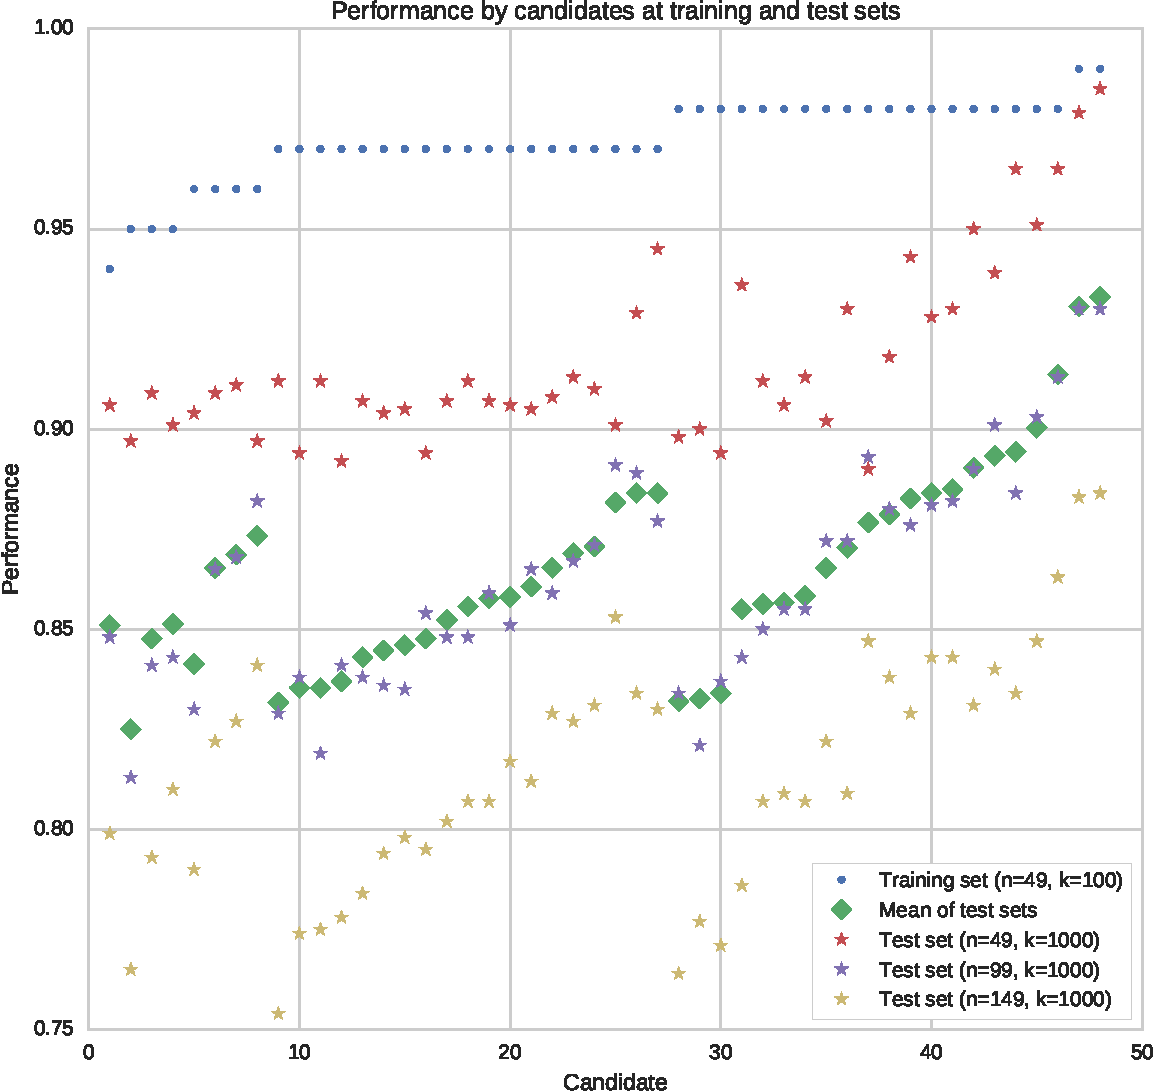
\includegraphics[width=\textwidth, keepaspectratio]{fig/sync_scores}
\caption[
    Performance of the 48 candidate solutions at the training and test sets.
]{
    Performance of the 48 candidate solutions at the training and test sets.
    The candidates have been ordered by training performance first, and average test performance second.
    }
\label{fig:sync_scores}
\end{figure}

Figure \ref{fig:sync_scores} shows the performance of the 48 candidates at the training set and each of the test sets.
It is clear that the candidates that have been trained on $n=49$
There is a correlation between the average score of the test sets and $n$, with the $n=49$ test performing closest to the $n=49$ training performance.
It is also clear that the two candidates that performed the best ($f=0.99$) at the training set, also perform the best at each of the test sets.


%\section{Firing Squad Synchronization Problem}
The \textit{firing squad synchronization problem} is an advanced task for multi-state 1D CA.
From a "resting" starting state the CA must be able to transmit signals so that at some point, every cell simultaneously enters the special "firing" state.

TODO

\section{Investigation of Genome Properties}
\label{sec:properties}
The process of running a task-solving experiments such as in the preceding sections is quite opaque.
The experiment is configured by human, but after it is started the system runs itself with no human input,
and the human observer can only wait and hope a useful result emerges at the end.

In order to gain a better understanding of the process,
an experiment was designed with the goal of investigating various properties of the population and their development over time,
rather than to solve a specific task.
This involves storing every single individual from the whole run, then analyzing them quantitatively afterwards.

CA-NEAT can be studied from multiple "angles": as a GA experiment there are properties such as fitness that can be studied,
as a CA experiment there is for example the $\lambda$ parameterization,
and as a graph-based encoding properties such as the number of nodes can be investigated.
Inspecting these, individually and trying to see correlation, should help with understand the system better,
and selecting better configurations for future experiments.

There are also multiple different mechanisms of the algorithm that can enabled or disabled by configuration.
Running multiple GA runs with different combinations of mechanisms enabled should give some indication about the effects of the mechanism.

\subsection{Experiment Design}
The "Swiss" morphogenesis task is used as the basis for this experiment,
since previous experiments with this problem showed it to be consistently solvable by CA-NEAT, but not trivially simple.
The fitness evaluation for morphogenesis problems is also very fast compared to other problems, making it possible to run tests with large populations in a reasonable amount of time.
The CA for this problem has $K=2$ cell states and the neighborhood shape "Von Neumann" ($N=5$) was used.
An initial population of size $P=1000$ was created, with $N$ input nodes, $K$ output nodes and no initial hidden nodes.
This same population was then used as the initial population for five independent "scenarios" of $G=100$ generations, with different mechanisms of NEAT in use.
Table \ref{tbl:NEAT_incremental} shows which mechanisms are in use in which scenario.
From top to bottom, the table can be read as gradually enabling mechanisms, until arriving at the full algorithm, as used in other experiments.

\begin{table}
    \centering
    \caption{Mechanisms enabled in different scenarios}
    \begin{tabular}{c|ccccc}
    Scenario & Mutation & Crossover & Selection pressure & Speciation & Elitism \\ \hline
    A   & \checkmark        & ~         & ~                  & ~          & ~       \\
    B   & \checkmark        & \checkmark         & ~                  & ~          & ~       \\
    C   & \checkmark        & \checkmark         & \checkmark                  & ~          & ~       \\
    D   & \checkmark        & \checkmark         & \checkmark                  & \checkmark          & ~       \\
    E   & \checkmark        & \checkmark         & \checkmark                  & \checkmark          & \checkmark       \\
    \end{tabular}
    \label{tbl:NEAT_incremental}
\end{table}

\begin{description}
\item[Scenario A] ~\\
Scenario A is different from the rest, since it is not a GA run, but more of a random walk in the search space using the mutation mechanism from the GA.
The individuals present in the initial population are mutated once per generation,
and the mutated versions are recorded as the next "generation".
With no crossover and no selection pressure, the individuals will be completely independent from each other throughout the entire run.
\item[Scenario B] ~\\
Scenario B uses NEAT, however the selection mechanism is completely randomized, so there is no selection pressure towards the goal of accomplishing the morphogenesis task.
\item[Scenario C] ~\\
Scenario C has selection pressure appropriate for the morphogenesis task, but does not use the speciation mechanism of NEAT.
\item[Scenario D] ~\\
Scenario D uses NEAT with selection pressure like C does, but also uses the speciation mechanism.
\item[Scenario E] ~\\
Scenario E uses all mechanisms of NEAT, including a per-species elitism degree of $E=1$.
\end{description}

Unlike the problem-solving experiments, this experiment does not involve multiple trials of the same configurations.
The reasoning is that this would mean we would be studying averages of averages in the following figures,
and some relationships between properties could be hidden by this.
We therefore should not draw any strong conclusions from the observations, but use it to find hypotheses that can be more rigorously investigated later.

\subsection{Fitness}
\begin{figure}
\centering
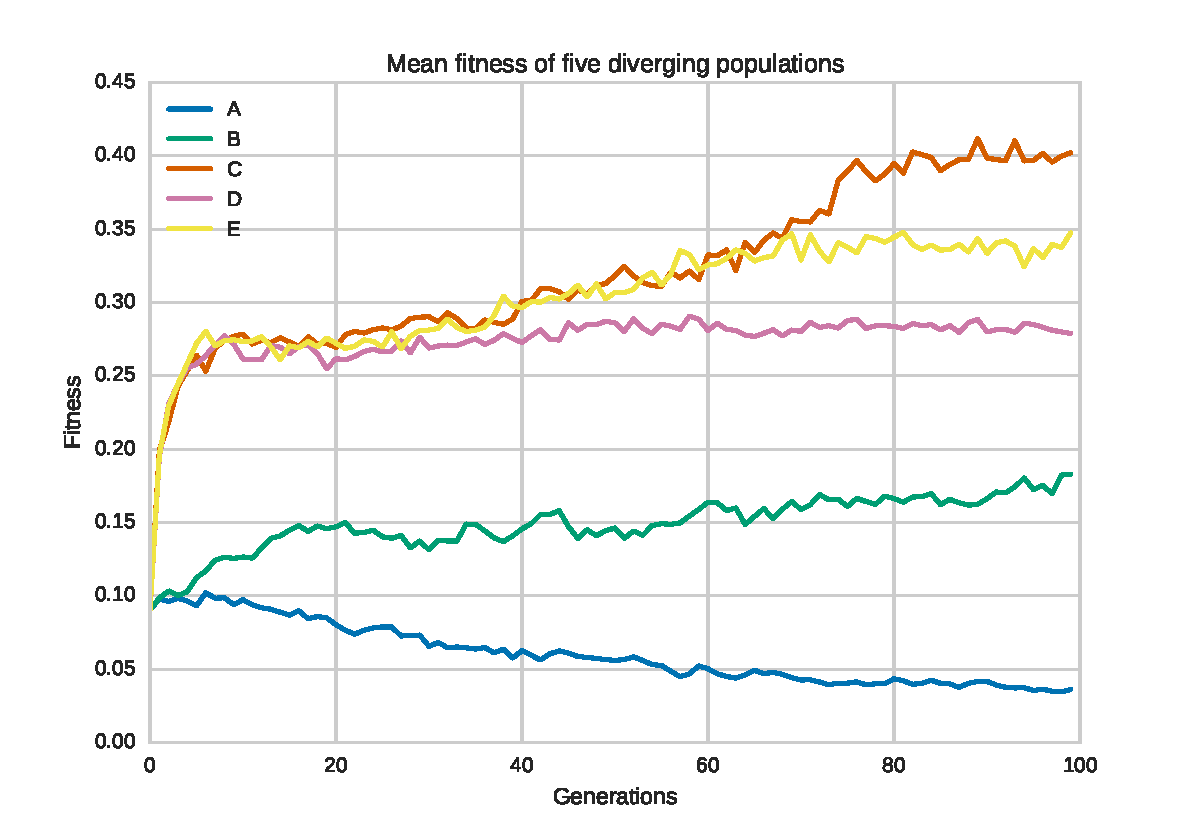
\includegraphics[width=\columnwidth]{fig/fitnesses}
\caption{The development over time of the mean fitness of the populations}
\label{fig:f_over_t}
\end{figure}

\begin{figure}
\centering
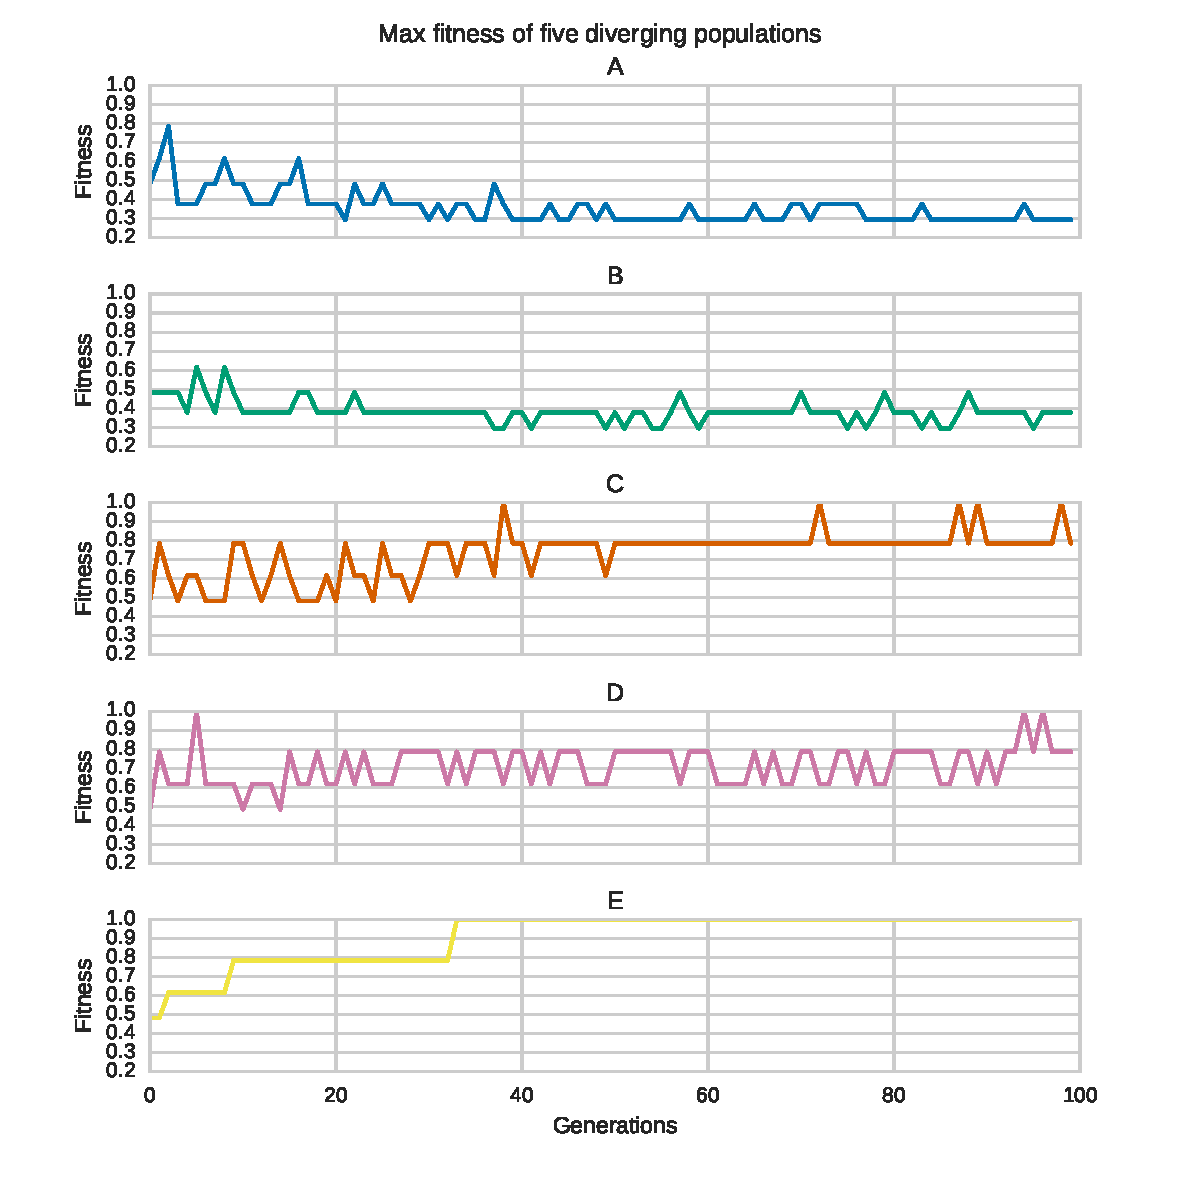
\includegraphics[width=\columnwidth]{fig/fitness_max}
\caption{The development over time of the max fitness of the populations}
\label{fig:max_fitness}
\end{figure}

When working with genetic algorithms, the most obvious property of a population to study is perhaps the average fitness over time.
Figure \ref{fig:f_over_t} shows the mean fitness development across the whole population for each of the five scenarios.
As one would expect, scenario A and B do not show any considerable improvement over time.
A declines steadily, while B has a slight, but not very significant increase.
Among C, D and E, which have selection pressure, there is a sharp increase in the first 10 generations.
D then flattens out for the remaining time, while C and E improves some more, at a slower rate.

Averaging hides one important aspect of the fitness distribution, namely the maximum value, which indicates "success" when it reaches $1.0$.
Looking at the maximum fitness development over time in Figure \ref{fig:max_fitness},
both A and B appears to decline over time, but B less so than A.
C and D act similar in that they hover around the upper half of the scale, sometimes finding a $1.0$ score, but are unable to stay stable there.
Whereas E, with the elitism mechanism is able to stay at $1.0$ once it finds it.
D finds a perfect solution quite early, but this seems likely to be a "fluke", since it losses it again and takes a long time to find another.
This is consistent with the results of the Swiss morphogenesis in Section \ref{sec:prev_work}, where in 100 independent trials, a few of them chanced upon an early solution.

The fact that the C average fitness overtakes both the D and E averages can hypothetically be explained by the difference the speciation mechanism makes.
In scenario C, the search can only optimize for fitness, so when it finds a good candidate it will make a large number of children for that candidate.
Scenarios D and E can optimize for diversity as well, searching in multiple directions.
When a good candidate is found in a species, its children will dominate only in that species,
while the other species continue their search unaffected.
Another possible factor is the stagnation check which is also part of the speciation mechanism.
This eliminates species that haven't improved average fitness in 15 generations.
If a species has "peaked", then it will be eliminated eventually, even if it's average fitness is above the population average.
In the task-solving experiments, the algorithm is stopped when a "perfect" solution is found, but in this experiment it is allowed to continue, so this effect can happen.

\subsection{Speciation}
\begin{figure}
\centering
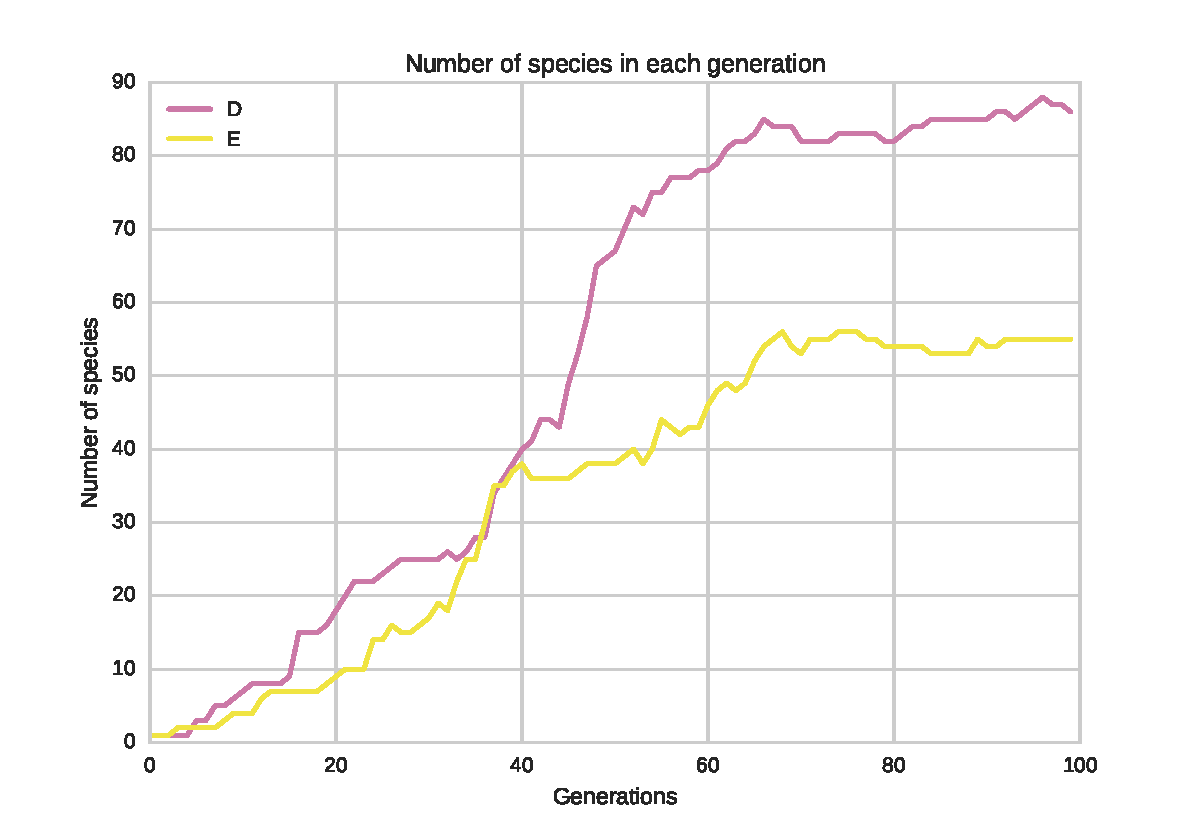
\includegraphics[width=\columnwidth]{fig/species}
\caption{The number of species in scenarios D and E over time}
\label{fig:species}
\end{figure}

\begin{figure}
\centering
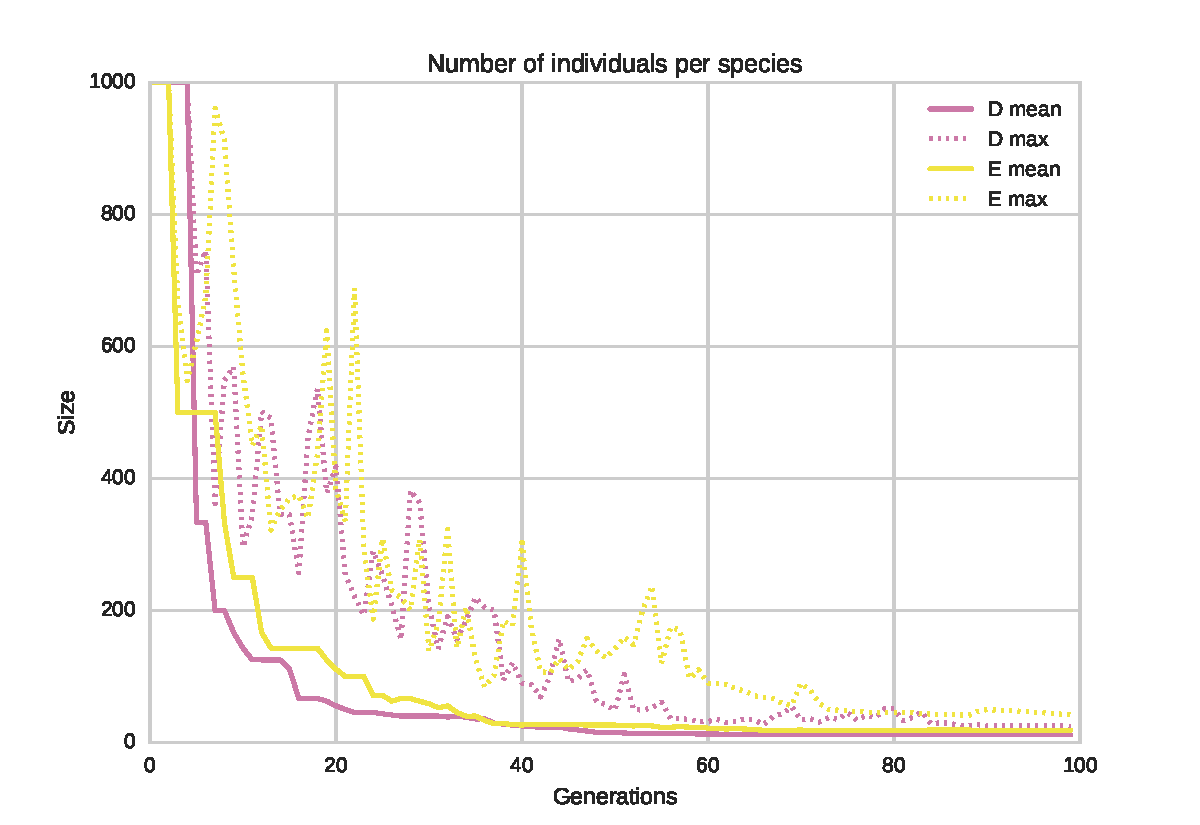
\includegraphics[width=\columnwidth]{fig/species_size}
\caption{The mean and max number of members in the species of scenarios D and E over time}
\label{fig:species_size}
\end{figure}

Another GA property that can be studied is the NEAT-specific speciation in scenarios D and E.
Figure \ref{fig:species} shows the number of different species over time.
Both follow approximately the same development in the first 40 generations, before D overtakes E and they stabilize at different levels.
The difference in levels is quite significant.
A speculative reason for this is that the lack of elitism in D means that a species there is more likely to split into multiple species by chance.
Whereas with elitism in E, the members of the species may be more likely to remain more similar to the elite in the population, leading to less diversity \textit{within} the species.

Figure \ref{fig:species_size} shows the mean number of members per species over time.
The development is as one would expect with the growing number of species seen in Figure \ref{fig:species}, declining more rapidly at first then gradually stabilizing.
The accompanying plot of the max number of species members gives an indication of the variance of the underlying data.
It fluctuates a lot at first, but as 100 generations approach,
the max stabilizes and is only slightly higher than the mean, indicating that the population consists of many species approximately the same (low) number of members.

In the case where there is elitism, as the species size approaches the number of elites ($E=1$) there is less room for innovation in that species, since one member of each species is always a copy of a previous one.
If the size were to reach $1$, there would be no innovation at all happening.
Since the population of scenario E seems to have stabilized around 55 species, a mean species size around $1000 / 55 \approx 18$ should avoid this problem and leave room for innovation.

\subsection{$\lambda$}
\begin{figure}
\centering
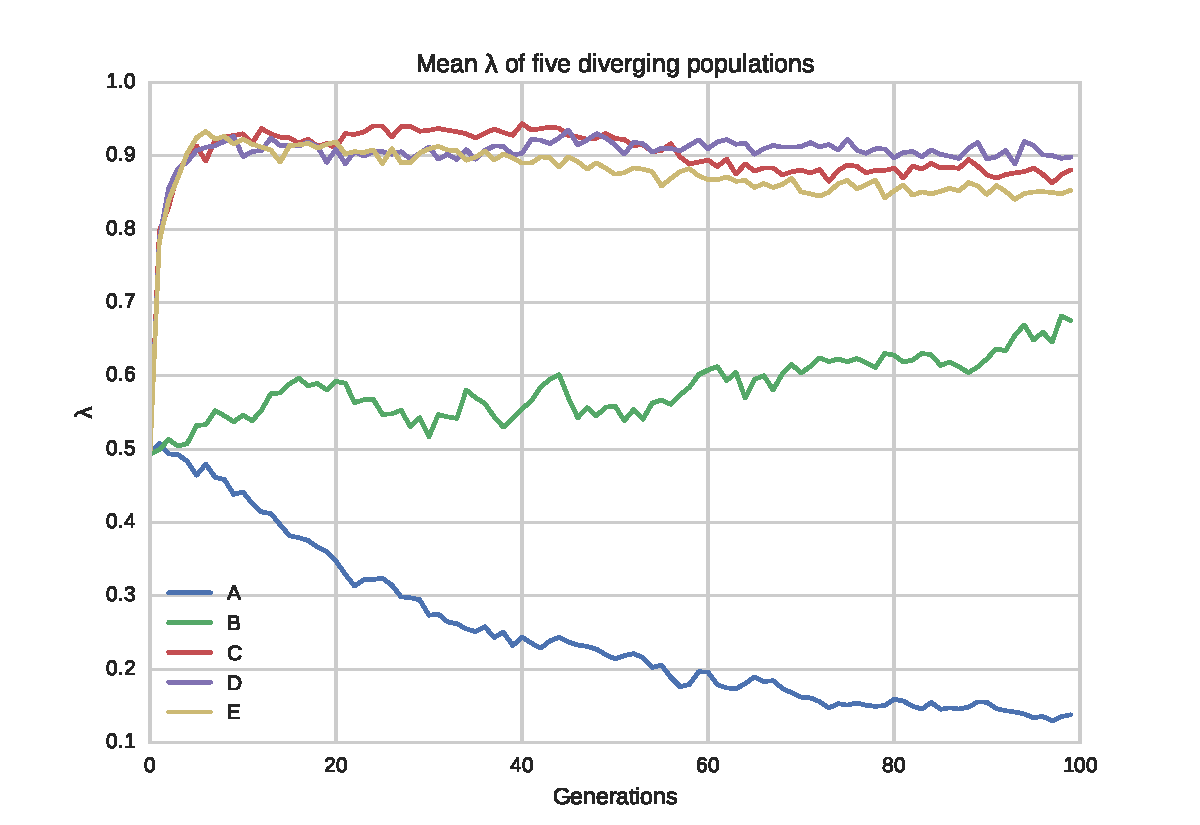
\includegraphics[width=\columnwidth]{fig/mean_lambda}
\caption{Development of the mean $\lambda$ of five scenarios over time}
\label{fig:lambda_over_t}
\end{figure}

\begin{figure}
\centering
\begin{subfigure}[t]{.49\columnwidth}
\centering
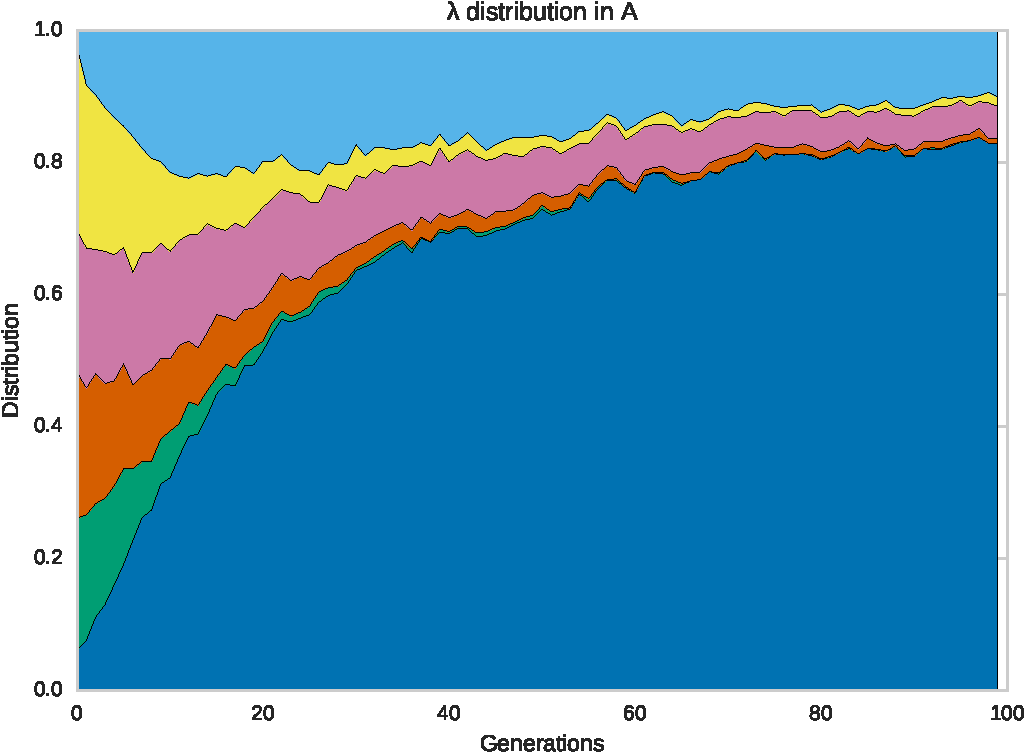
\includegraphics[width=\columnwidth]{fig/lambda_A}
\caption{Scenario A}
\label{fig:lambda_A}
\end{subfigure}
\begin{subfigure}[t]{.49\columnwidth}
\centering
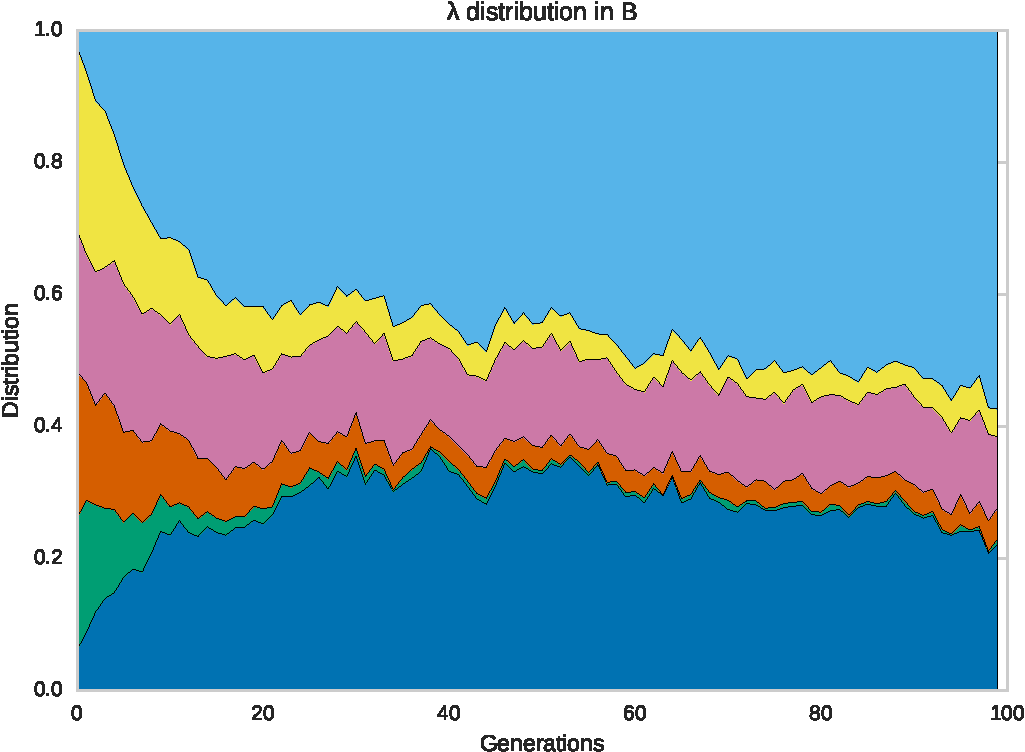
\includegraphics[width=\columnwidth]{fig/lambda_B}
\caption{Scenario B}
\label{fig:lambda_B}
\end{subfigure}
\begin{subfigure}[t]{.49\columnwidth}
\centering
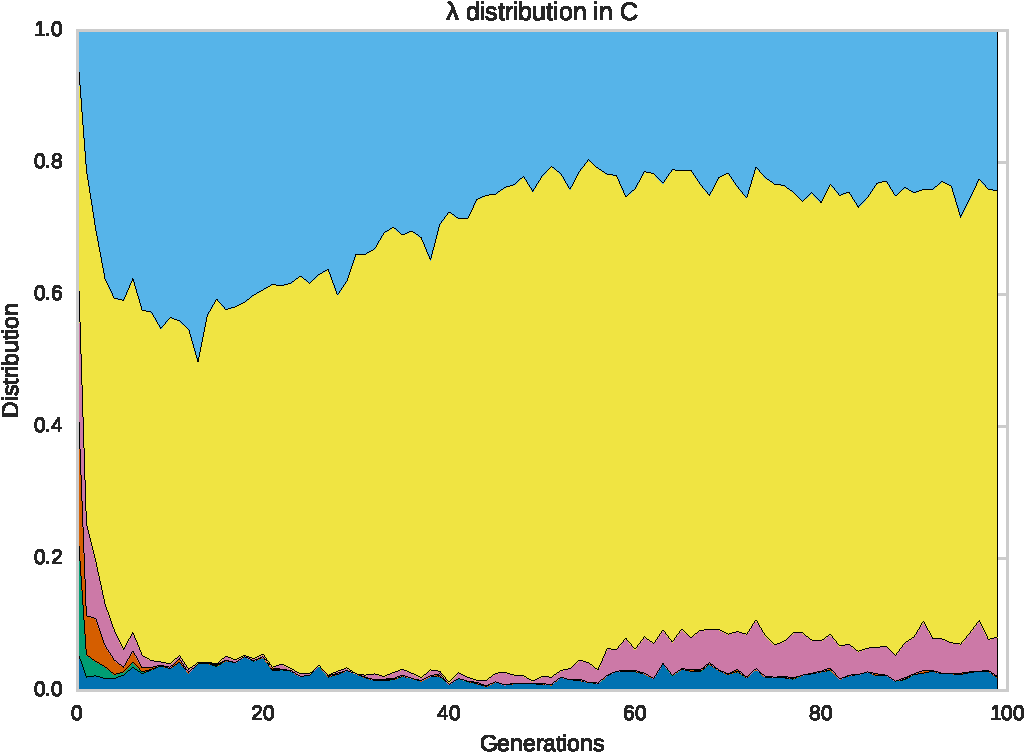
\includegraphics[width=\columnwidth]{fig/lambda_C}
\caption{Scenario C}
\label{fig:lambda_C}
\end{subfigure}
\begin{subfigure}[t]{.49\columnwidth}
\centering
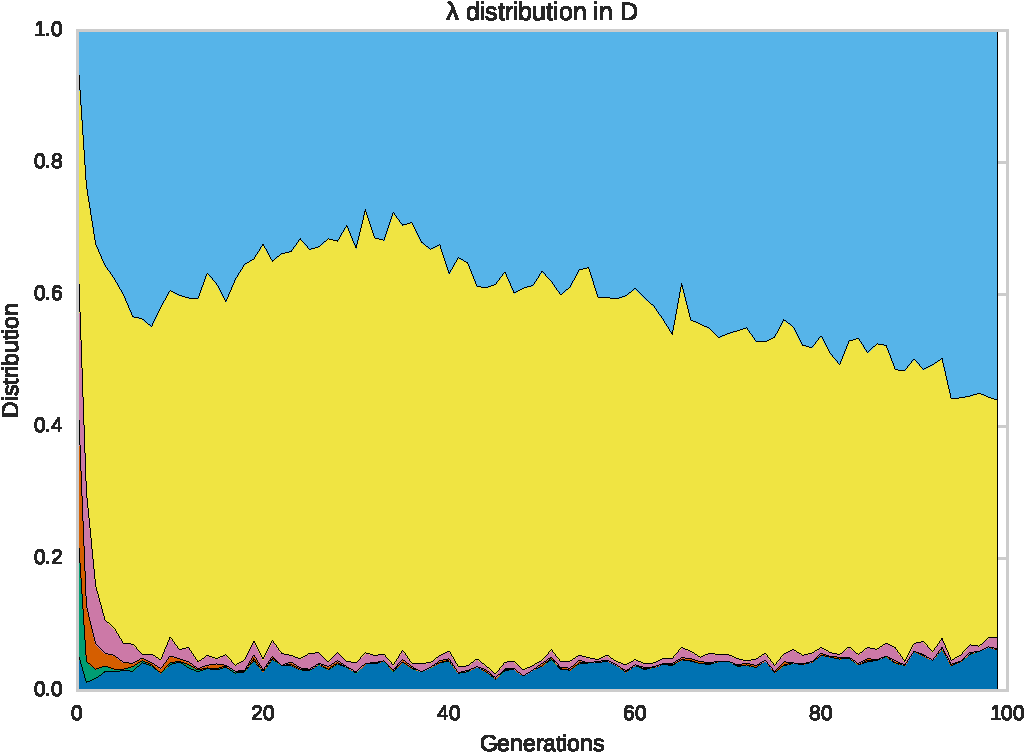
\includegraphics[width=\columnwidth]{fig/lambda_D}
\caption{Scenario D}
\label{fig:lambda_D}
\end{subfigure}
\begin{subfigure}[t]{.49\columnwidth}
\centering
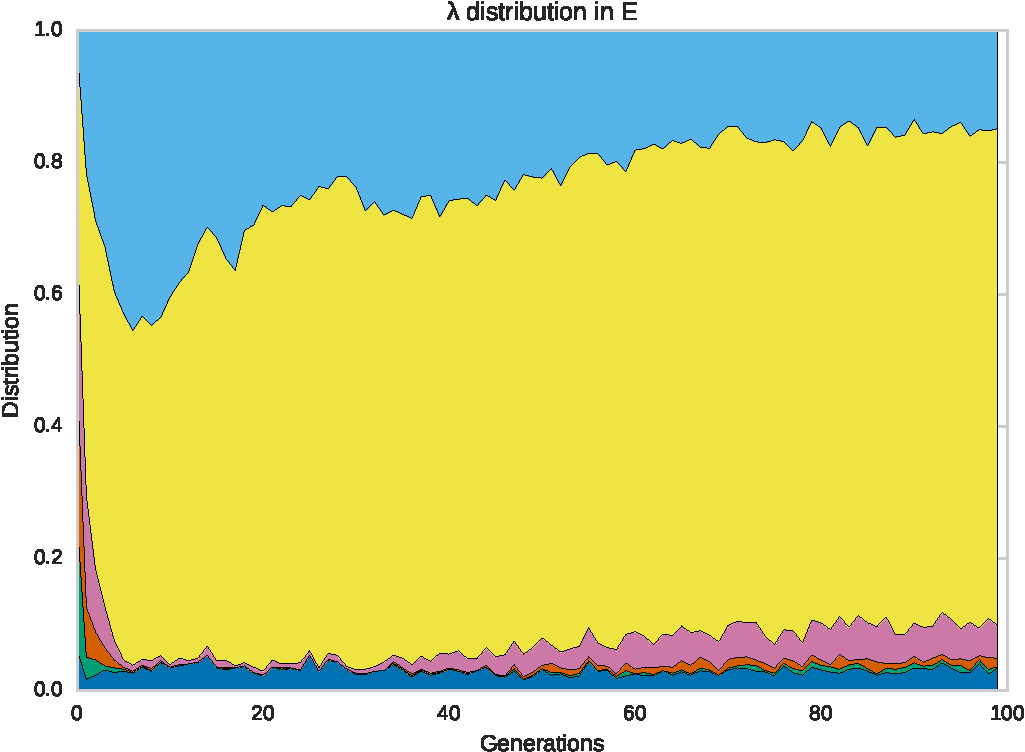
\includegraphics[width=\columnwidth]{fig/lambda_E}
\caption{Scenario E}
\label{fig:lambda_E}
\end{subfigure}
\begin{subfigure}[t]{.49\columnwidth}
\centering
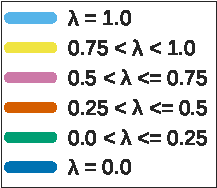
\includegraphics[width=\columnwidth, height=4.5cm, keepaspectratio]{fig/lambda_legend}
\caption{Legend}
\end{subfigure}

\caption{Breakdown of $\lambda$ distribution over time in five scenarios}
\label{fig:lambdas_breakdown}
\end{figure}

The $\lambda$ parameter is an interesting property of a CA transition function to study.
Figure \ref{fig:lambda_over_t} shows the mean $\lambda$ over time for the five scenarios.
The shapes of the curves have a lot of similarities with the shapes of the fitness curves in Figure \ref{fig:f_over_t}.
The random mutation in scenario A drives the mean $\lambda$ towards $0$,
while the combination of mutation and crossover without selection pressure of scenario B causes the $\lambda$ to fluctuate a lot and increase slightly, but not very significantly.
Scenarios C, D and E have roughly the same development: a sharp rise to about $0.9$, then flattening out.
%Both D and E do a slight "correction" afterwards, slowly decreasing after the initial rapid rise.

Figure \ref{fig:lambdas_breakdown} shows the scenarios broken down individually into stack plots, illustrating the distribution of values changing over time.
The values are sorted into six bins, two special ones for $\lambda$ exactly equal to $0.0$ and $1.0$ and four for the equal intervals in between.
In earlier experiments it was observed that the two extreme $\lambda$ occur often, so they get special bins in this visualization.

It can be seen that the scenario A has a very strong bias towards producing $\lambda = 0.0$,
while the other scenarios skew more towards producing higher $\lambda$ values.
This would suggest that crossover mechanism is at least partially responsible for producing higher $\lambda$ values.
There is also a strong resemblance between C and E, less so between D and the others.
Why this is so is not entirely obvious, but it could just be a consequence of the randomness of the trial.
If the experiment was repeated with multiple trials, we could determine if this is just a fluke or not.
In any case, it is clear that all the scenarios with selection pressure are strongly biased towards producing $\lambda > 0.75$.

The task at hand and the implementation of the fitness function must also be considered when analyzing the $\lambda$ result.
The fitness evaluation function is described in detail in Section \ref{sec:morph_problems}.
Notably, when trying to produce a "Swiss flag" pattern, 
$20/25$ cells are active in the target state, meaning that the algorithm can get \textit{some} score easily by producing a transition function with $\lambda = 1.0$.
This can explain why the algorithm produces very many $\lambda=1.0$ solutions early on.
%Considering this, as well as Langton's theory of the "Edge of Chaos", the breakdowns seen in C, D and E make sense.

%\begin{figure}
%\centering
%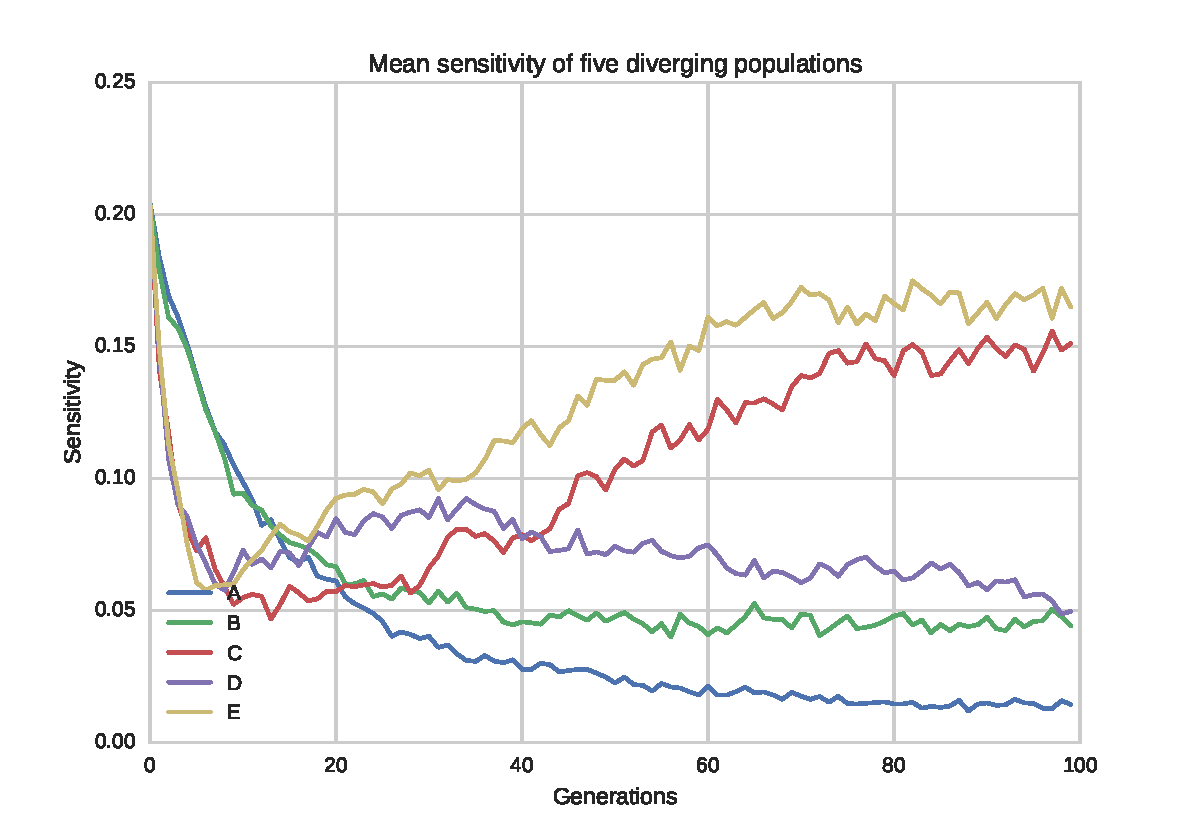
\includegraphics[width=\columnwidth]{fig/sensitivity}
%\caption{TODO}
%\label{fig:sensitivity}
%\end{figure}

%\begin{figure}
%\centering
%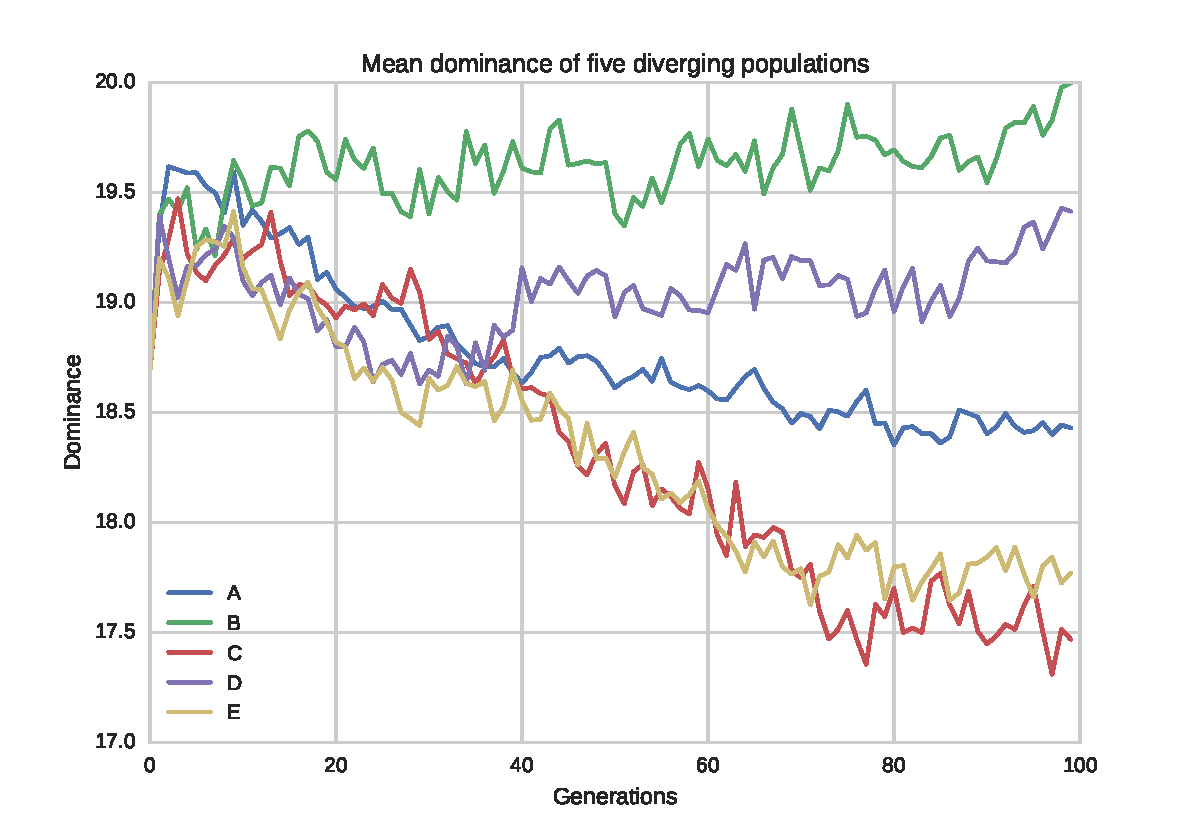
\includegraphics[width=\columnwidth]{fig/dominance}
%\caption{TODO}
%\label{fig:dominance}
%\end{figure}


\subsection{Distinct behaviors}
\begin{figure}
\centering
\includegraphics[width=\columnwidth]{fig/unique_behaviors}
\caption{Number of unique behaviors in each generation}
\label{fig:unique_behaviors}
\end{figure}

\begin{figure}
\centering
\includegraphics[width=\columnwidth]{fig/cummulative_unique_behaviors}
\caption{
    Number of unique behaviors seen over time, cumulative.
}
\label{fig:cummulative_unique_behaviors}
\end{figure}

\begin{figure}
\centering
\includegraphics[width=\columnwidth]{fig/cummulative_unique_perfect}
\caption{
    Number of unique $f=1.0$ behaviors seen over time, cumulative.
}
\label{fig:cummulative_unique_perfect}
\end{figure}

%\begin{figure}
%\centering
%\includegraphics[width=\columnwidth]{fig/mutation_behavior_change}
%\caption{Ratio of genotypes that change behavior after mutation}
%\label{fig:mutation_behavior_change}
%\end{figure}

%Studying the $\lambda$ parameter can give some insights, but it does not capture every aspect of the transition function behavior.
Another way to analyze the population is to look at the diversity of the enumerated behavior "strings" over time.
Figure \ref{fig:unique_behaviors} shows how many unique behaviors are present in each generation of each scenario.
The initial population is clearly very diverse, but the diversity drops very rapidly in each of the scenarios.
Scenarios A and B decrease slightly slower than the rest at the beginning.
The rate of decreasing slows down and they eventually stabilize at low levels.
Scenarios C, D and E drop down fast at first, but then they do a sharp turn.
C and D fluctuate a it up and down, but overall seem to stabilize.
E rises steadily again and stabilizes at a significantly higher level than the others.

Figure \ref{fig:cummulative_unique_behaviors} visualizes the number of unique behaviors seen in the entire lifetime of the scenario.
A and B are almost identical, showing almost no increase after the first 20 generations.
C and D climb steadily and overtake A and B at different points.
The contrast between E and the rest is stark.
There is a much higher rate of increase, and it is almost linear over time, reaching about twice the value that the next best does in 100 generations.
These result have some big implications.
First of all, it is clear that a random search such as A and B gets "stuck" quite quickly and stops producing innovative results.
With selection pressure, the search is slower at first, needing quite some time to overtake the initial flood of innovation produced by randomness.
But it keeps a steady increase where the random search stops.
And the presence of elitism increases the innovation by a very considerable degree.

In a "best-case" where every behavior in every generation is distinct,
the number of unique behaviors observed would be $P * G = 100000$.
Scenario E passes 12000 unique behaviors observed, which is "only" 12\% of the theoretical maximum.
And for a $K=2, N=5$ CA, the number of total possible behaviors is $K^{K^N} = 2^{32} \approx 4.3 * 10^9$.
This illustrates the futility of attempting to solve advanced CA tasks by exhaustive enumeration of behaviors.
Luckily, while the proverbial haystack may be humongous,
there are many needles to be found within it, and you only need to find one to be successful.
Figure \ref{fig:cummulative_unique_perfect} illustrates the number of distinct behaviors observed with a perfect fitness score.
As one might expect, the diversity of the optimal behaviors is higher when the diversity of all behaviors is higher.
Scenario E is able to find 7 distinct solutions to the task.

\subsection{Network Topology}
\begin{figure}
\centering
\includegraphics[width=\columnwidth]{fig/sizes}
\caption{The mean number of nodes in each scenario}
\label{fig:sizes}
\end{figure}

\begin{figure}
\centering
\includegraphics[width=\columnwidth]{fig/vestigial_nodes}
\caption{The mean number of disconnected nodes in each scenario}
\label{fig:vestigial_nodes}
\end{figure}

%\begin{figure}
%\centering
%\includegraphics[width=\columnwidth]{fig/vestigial_ratio}
%\caption{The ratio of connected nodes in each scenario}
%\label{fig:vestigial_ratio}
%\end{figure}

\begin{figure}
\centering
\includegraphics[width=\columnwidth]{fig/connectivity}
\caption{The mean connectivity degree in each population}
\label{fig:connectivity}
\end{figure}

The individuals of the populations are graph structures, and can also be studied as such.
Figure \ref{fig:sizes} shows the development of the mean number of nodes in the networks of each scenario.
The growth of scenario A is approximately linear.
Since the individuals of the population are completely independent from each other,
the law of large numbers means that the curve should fit the expected value given by the probabilities of adding and removing nodes, $(P_\text{add} - P_\text{remove})x = (0.5 - 0.25)x = 0.25x$.
This is not a very useful insight by itself, but it does give a baseline which the other scenarios can be compared to.
Scenario B has a slightly higher growth than A.
This makes sense considering the crossover mechanism.
If two parents independently are likely to gain a new node, then their child will have both of the new nodes, leading to a bigger growth rate overall.
The three scenarios with selection pressure at first follow the same pattern, with much lower growth than the baseline.
Then they diverge around 30 generations.
Scenario C "catches up" with scenario A and settles into a near-linear growth like scenario A.
Scenario D also goes into a linear growth close to the same as scenario A, but without "catching up" first.
Scenario E continues with almost the same growth rate for all 100 generations, ending up at a much lower number than the rest.

Figure \ref{fig:vestigial_nodes} shows the number of "vestigial" nodes that do not connect to the output layer.
The significance of these is that they are equally likely to be affected by mutation as any other node, but they do not affect the output of the network.
The more vestigial nodes there are, the more likely that the mutation operation does "nothing".

Scenarios A and B have curve shapes very similar to those they had in Figure \ref{fig:sizes}, suggesting a simple proportional correlation when the process is completely random.
More interestingly, the curve of scenario C does a sudden turn to overtake both A and B.
The curve of C reaches almost the same value as that in Figure \ref{fig:sizes}, indicating the population members have a very large number of disconnected nodes.
The curves of D and E are similar to their counterparts in Figure \ref{fig:sizes}.
Again it is clear that E has a distinctly different development than the rest.

%Figure \ref{fig:vestigial_ratio} shows the relationship between Figures \ref{fig:sizes} and \ref{fig:vestigial_nodes}.
%Scenarios A and B run a very parallel course here, as does D and E.
%The four actually end up near the same value at 100 generations.
%C on the other hand, goes off to do its own thing completely here, and as noted earlier, ends up at a very low ratio of connectedness.

Figure \ref{fig:connectivity} shows another measure of connectedness which is often used in graph theory, $\text{connectivity} = \frac{c}{\sum_{x=1}^{n}{x}}$, where $c$ is the number of connections and $n$ is the number of nodes.
In this perspective, C follows D and E at first, but diverges and drops much quicker to the level of A and B.

What these observations seem to indicate, is that the population of C comes to be dominated by networks with many nodes and fewer connections.
It is likely that in repeated trial this would not occur every time, but that it is just part of the randomness of the single trial.
This is perhaps more likely to occur with the scenario C parameters than the others.
Scenarios A and B are somewhat predictable systems with behavior determined by the constant parameters set before the experiment.
The selection pressure of C can possibly act as a feedback loop, causing a random feature to dominate the whole population.
Scenarios D and E have speciation which automatically create (somewhat) independent trials within the population.

TODO round off this section with some overarching general discussion, maybe in the next chapter

\section{Novelty Search}
Section \ref{sec:novelty} describes how CA-NEAT was extended to support novelty search.

Because novelty search disregards the objective,
a search for a specific neighborhood size $N$ and number of states $K$ creates population that can be used on any CA with that $N$ or $K$.
For example, the same population could contain solutions to both morphogenesis and replication of both the 6x6 "Tricolor" and 7x7 "Nordic" patterns (Figure \ref{fig:patterns}).

\subsection{Results}
\begin{figure}
\centering
\includegraphics[height=0.4\textheight, width=\textwidth, keepaspectratio]{fig/novelty_diversity}
\caption[
    Cumulative number of unique behaviors observed
]{
    Cumulative number of unique behaviors observed.
    The two runs share the properties $N=5, K=4, P=50, G=1000$, and differ in whether they have speciation enabled.
}
\label{fig:novelty_diversity}
\end{figure}

\begin{figure}
\centering
\includegraphics[height=0.4\textheight, width=\textwidth, keepaspectratio]{fig/innovation_archive_size}
\caption[
    Size of the innovation archives
]{
    Size of the innovation archives.
    The archives are a subset of their corresponding populations.
}
\label{fig:innovation_archive_size}
\end{figure}

\begin{table}
\centering
\caption{Overview of the novelty search runs attempted}
\begin{tabular}{c|c|c|c|c|l}
    N   &   K   &   P   &   G   &   Speciation  &   Objectives tested   \\\hline
    5   &   4   &   50  &   1000    &   Yes &   \{Swiss, Nordic\} \{morphogenesis, replication\} \\
    5   &   4   &   50  &   1000    &   No  &   \{Swiss, Nordic\} \{morphogenesis, replication\} \\
    5   &   2   &   50  &   1000    &   No  &   Border morphogenesis \\
    7   &   2   &   200 &   1000    &   No  &   Majority, synchronization
\end{tabular}
\label{tbl:novelty}
\end{table}

Several different $N$ and $K$ combinations were tested and the resulting innovations archives checked against the objective function of appropriate tasks.
Table \ref{tbl:novelty} gives an overview of the combinations tested.
When testing against the appropriate objective functions, the results were not particularly useful, with no optimal solutions found for any of the tasks tested.
Detailed results about the fitnesses found are not too interesting and is omitted from this report.
Suffice it to say, the success rate was 0\% across the board.

One configuration that was tested was $N=5$, $K=4$, a population size of $P=50$, for $G=1000$ generations.
We will take closer look at the results, assuming them to be representative for the results of all the experiments.
This configuration was tested in two independent runs, with and without speciation.
Figure \ref{fig:novelty_diversity} shows the cumulative number of unique behaviors observed in the two runs.
The figure is created from the full population of each run, not the innovation archive, which is a subset of the full population.
It shows that the novelty search is correctly implemented and does in fact produce many novel genotypes in each generation.
It can be compared to Figure \ref{fig:cummulative_unique_behaviors} in Section \ref{sec:properties}, taking into account the different population size
The curves are approximately equal, showing no particular effect from the presence or lack of speciation.
At 1000 generations, the runs are at 47806 unique individuals (no speciation) and 47969 (with speciation).
This is as good as equal, and it is close to the curve of the maximum possible unique behaviors $y(x)=50x$.
Still, $50000$ unique individuals would still only be $\frac{50000}{2^{2^{5}}} \approx 0.0012\%$ of the search space.

Figure \ref{fig:innovation_archive_size} shows the development of the sizes of the innovation archives.
The two archive sizes are approximately the same in the first 150 generations, but then diverge considerably.
The population without speciation adds much fewer innovations to the archive than the population with speciation does.
Over 1000 generations, the population with speciation adds on average almost 10 individuals to the archive per generation,
while the population with speciation adds on average 3-4 innovations per generation.
Since the speciation threshold is supposed to dynamically adjust to keep the number of added innovations between 1-5,
this must mean that the average innovation metric in the population is changing a lot, so that the threshold is not able to keep up.
This could happen because the average innovation degree is continuously increasing, or because it is fluctuating around some value.
In either case the threshold adjusting algorithm is always a step behind.

Because of performance issues with the implementation,
it was not feasible to run many independent trials of the same configuration.
There is a possibility that in a larger number of trials, some might succeed.
But a more performant implementation is necessary to test this.

These results suggest that this approach to novelty search is not going to lead to produce anything that is more interesting than what objective search produces.
This does not necessarily mean that novelty search is never going to work for CA problems, only that the setup used in these experiments is flawed and must be reconsidered.


\cleardoublepage
%\chapter{Results}
TODO


%\cleardoublepage
\chapter{Discussion}
TODO


\cleardoublepage
\chapter{Conclusion}
TODO


\cleardoublepage

%% PART 4
\pagestyle{fancy}
\fancyhf{}
\renewcommand{\chaptermark}[1]{\markboth{\chaptername\ \thechapter.\ #1}{}}
\renewcommand{\sectionmark}[1]{\markright{\thesection\ #1}}
\renewcommand{\headrulewidth}{0.1ex}
\renewcommand{\footrulewidth}{0.1ex}
\fancyfoot[LE,RO]{\thepage}
\fancypagestyle{plain}{\fancyhf{}\fancyfoot[LE,RO]{\thepage}\renewcommand{\headrulewidth}{0ex}}

\addcontentsline{toc}{chapter}{Bibliography}

%\bibliographystyle{elsarticle-harv}
\bibliographystyle{elsarticle-num}
\bibliography{bibliography}

\cleardoublepage

\section*{\begin{center}{\Huge Appendix}\end{center}}
\addcontentsline{toc}{chapter}{Appendix}
$\\[0.5cm]$

\noindent Write your appendix here...

\end{document}
